\chapter{Topic Extraction: identifying topics from tags}
\doublespacing
\label{chap:ttd}
\minitoc

\section{Topic Trees Distributions (TTD)}\label{sec:TTD}
\label{sec:empirical}

\subsection{Problem Definition: mining topics and communities}
% TODO: add a paragraph explaininh the link with previous chapter and itroducing the need for this new chapter e.g. classical LDA is too slow.
%DONE
In Chapter \ref{chap:qasm}, we mentioned that there are two kinds of information in user-generated content. One of them is latent information such as topics and communities, which are not explicitly existed in the original data set. In this chapter, we aim at extracting these latent information from tags on Q\&A sites.

In Chapter \ref{chap:lda}, we applied the original LDA model and we found it is complicated and slow to extract these latent information. In this chapter, we aim at proposing a much simple and efficient method to extract these information. 

% TODO: do not repeat what was said in prvious chapter e.g. the definitions should be given once in the whole thesis.
% TODO: the previous TODOs applay to all chapters
Many sites supporting user-generated content let their members organize their contributions with tags. The social tagging approach also applies to Q\&A platforms. In particular, in StackOverflow, a user submits a question, then assigns 1$\sim$5 tags to indicate the topics of the question. Other users who are interested in the question may provide answers to the question. As the tags attached to a question can reflect its topic, users asking the question can be considered as interested by its topic and users successfully answering a question can be considered as experts in that topic.

Let $U=\{u_1,u_2...u_n\}$ be the set of users, $Q=\{q_1,q_2...q_m\}$ the set of questions and $T=\{t_1,t_2...t_v\}$ the set of tags. We aim at:

\begin{enumerate}
 \item extracting topics distribution $Topic=\{topic_1,topic_2...topic_k\}$ from $T$, and for each $topic_k$, defining $topic_k=\{p_{k1},p_{k2}...p_{kv}\}$ where $p_{ki}$ denotes the probability of tag $t_i$ to be related to $topic_k$; an then
  \item detecting user's interests. For a user $u_i \in U$, we define $I_i=\{I_{i1},I_{i2}...I_{ik}\}$ where $I_{ik}$ denotes the probability of $u_i$ to be interested in $topic_k$.
\end{enumerate}


\subsection{First-Tag Enrichment: adding a more general tag when needed}
When sorting the tags of a question by their global frequency, we found that normally the first tag of a question is much more general and indicates the domain of the question. For example, a question tagged with \{\textit{c\#}, \textit{iostream}, \textit{fstream}\} is related to \textit{c\#}; a question tagged with \{\textit{html}, \textit{css}, \textit{height}\} is related to \textit{html}. However, there are also some questions which have less tags and, in this case, the tags are less popular, like a question tagged with \{\textit{ant}\} or a question tagged with \{\textit{qt}, \textit{boost}\}. For these questions, the main domain is implicit. Our experiment dataset shows that nearly $12\%$ of the questions only have one tag, and nearly $25\%$ of the questions only have two tags.

% TODO: justify the heuristics, do you have the metrics we talked about eg correlation between frequency and rank ?    


Therefore, we propose an approach to enrich a question with a first tag when needed. The first step of our approach consists in computing the first-tag distribution.
\begin{figure}[htp]
\centering
%\epsfig{file=fly.eps, height=1in, width=1in} % use this if you use "pdflatex"
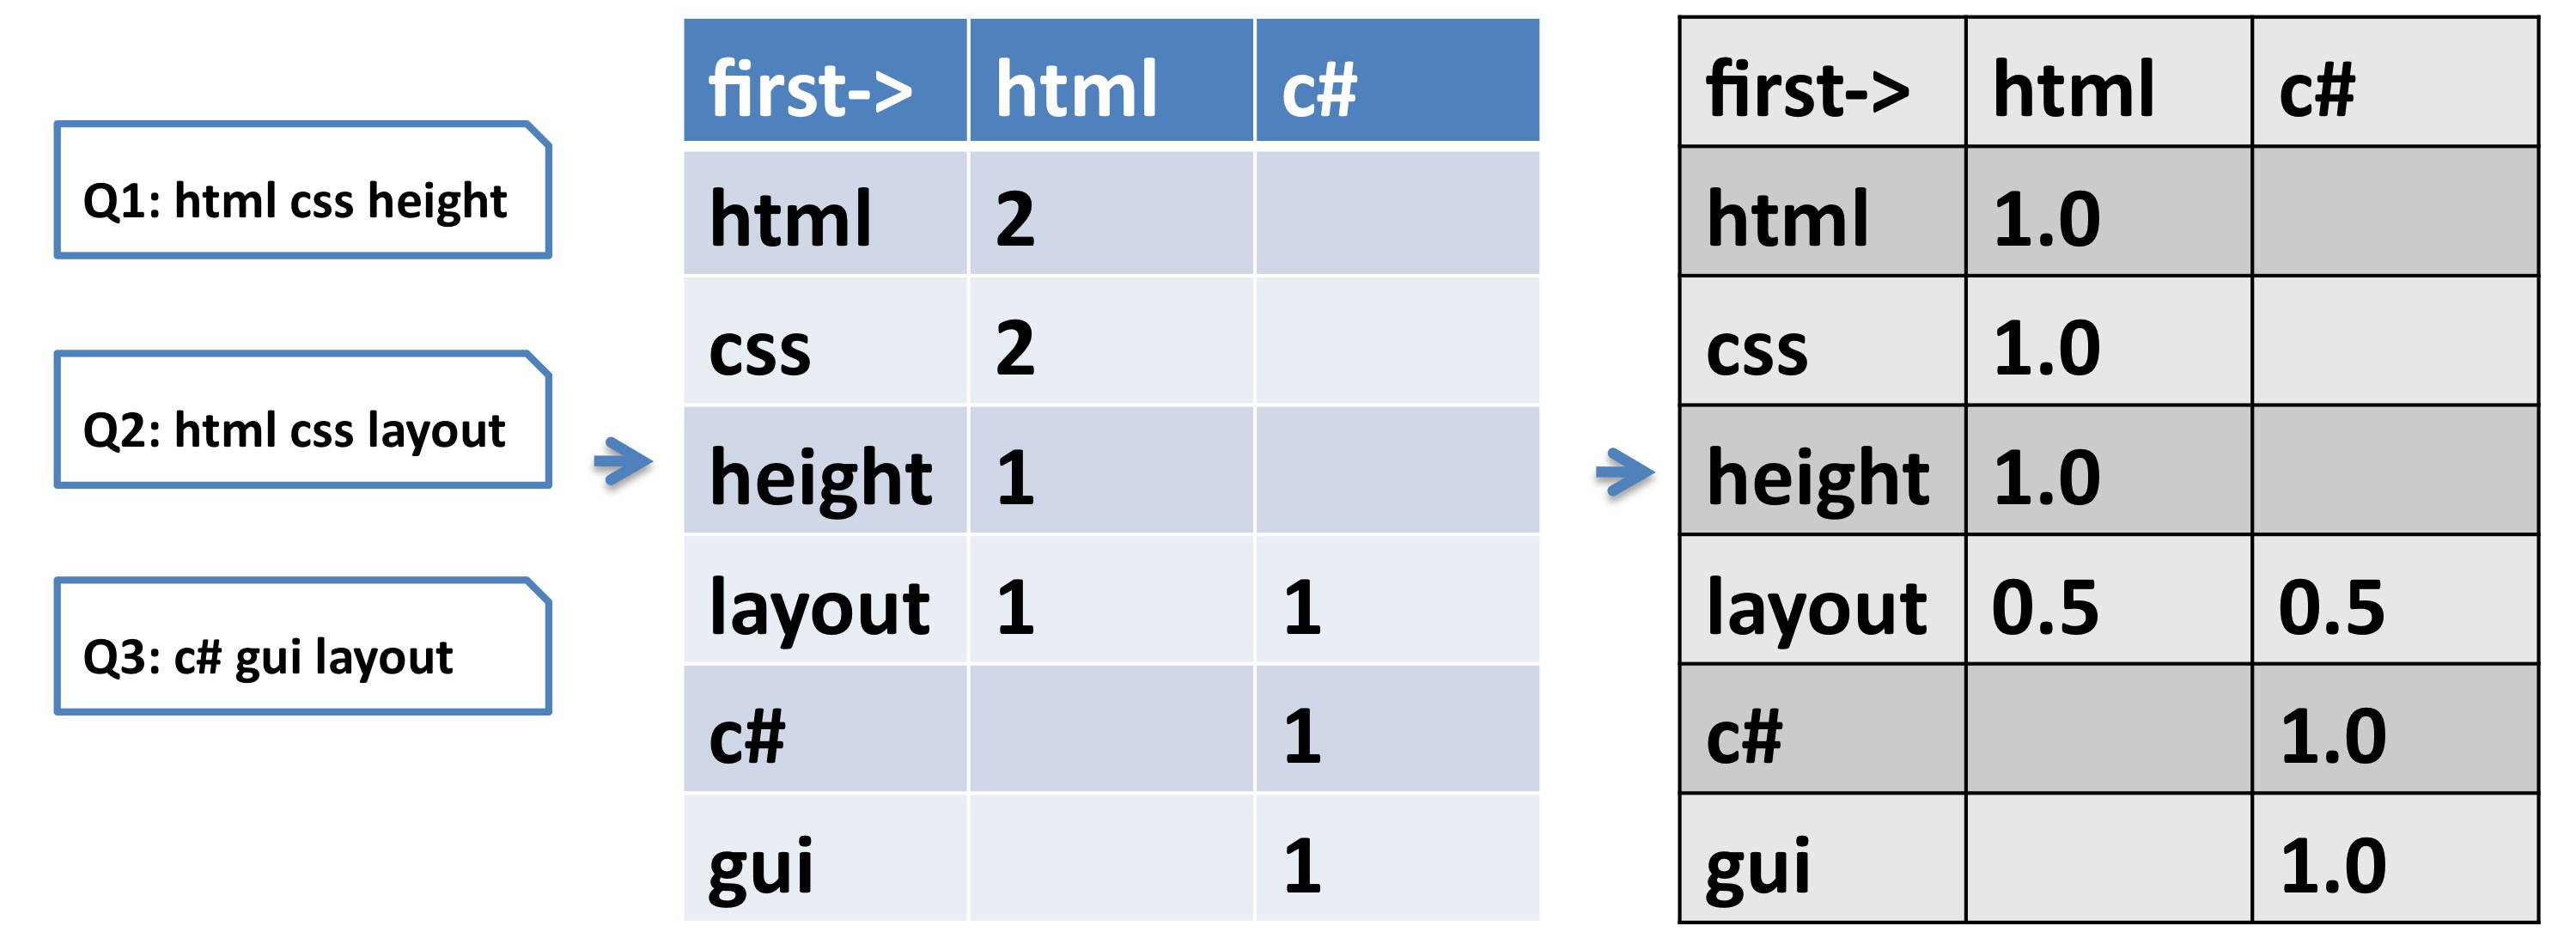
\includegraphics[width=5in]{7.jpg}  
\caption{Example of computing a first-tag distribution}
\label{fig:examplefirsttag} 
\end{figure}
For example, as shown in Figure \ref{fig:examplefirsttag}, let us consider the three tag lists, \{\textit{html}, \textit{css}, \textit{height}\},  \{\textit{html}, \textit{css}, \textit{layout}\}, and \{\textit{c\#}, \textit{gui}, \textit{layout}\}, respectively associated to questions Q1, Q2, Q3 . The first-tag frequency map for \textit{html} is \{\textit{html}:2\}, the first-tag frequency map for \textit{css} is \{\textit{html}:2\}, and the first-tag frequency map for \textit{layout} is \{\textit{html}:1,\textit{c\#}:1\}. Given a tag, the probability of its first-tag is computed by equation \ref{eq:firsttag}, which is the Maximum Likelihood estimation (MLE) of the probability $p(T_f|T_i)$, where $I(T_i)$ denotes the occurrence of tag $T_i$ and $I(T_f,T_i)$ denotes the co-occurrence of first-tag $T_f$ and tag $T_i$.

\begin{equation}
%\scriptsize
\begin{split}
p(T_f|T_i)  &=\frac{p(T_f,T_i) }{p(T_i)} \\
                  &\propto \frac{I(T_f,T_i)}{I(T_i)}
\label{eq:firsttag}
\end{split}
\end{equation}


We compute the probabilities just by normalizing the first-tag frequency map. In the previous example, the first-tag frequency map for \textit{css} becomes \{\textit{html}:1.0\} and the first-tag frequency map for \textit{layout} becomes \{\textit{html}:0.5, \textit{c\#}:0.5\}. In order to lower the probabilities of low frequency tags as first-tag, we use the squashing function \ref{eq:normalize}:

%TODO : you equations should use proper mathematical notation for sums, you should define p(Tf,Ti) and define a frequency function for tags and for tag pairs ; here it is not easy to see over what set you sum
%DONE


\begin{equation}
\begin{split}
p(T_f|T_i) &=\frac{I(T_f,T_i)}{I(T_i)}*\sigma(I(T_f)) \\
                  %&=\frac{record\_freq}{sum(record\_freq)} 
                  &\propto \frac{I(T_f,T_i)}{I(T_i)}*\frac{1}{(1+e^{-k*I(T_f)})}
\label{eq:normalize}
\end{split}
\end{equation}

where, $I(T_f)$ denotes the frequency of \textit{first-tag}. $I(T_f,T_i)$ denotes the co-occurrence of \textit{first-tag} and \textit{tag}, $I(T_i)$ denotes the frequency of \textit{tag}  $\sigma(x)$ is sigmoid function, which is used as a squashing function for numerical stability. The value of sigmoid function is between 0 and 1, however the shape of this function is largely determined by parameter $k$. Considering the maximum value of tag frequency (tag c\#:$31,801$) in our dataset, we chose $k$ as 0.001 (dotted line), which will lower the probabilities of low frequency tags as first-tag while maintaining the probabilities of high frequency tags as first-tag. Figure \ref{fig:sigmoidfunction} recalls the shape of the sigmoid function for different values of $k$.

\begin{figure}[htp]
\centering
%\epsfig{file=fly.eps, height=1in, width=1in} % use this if you use "pdflatex"
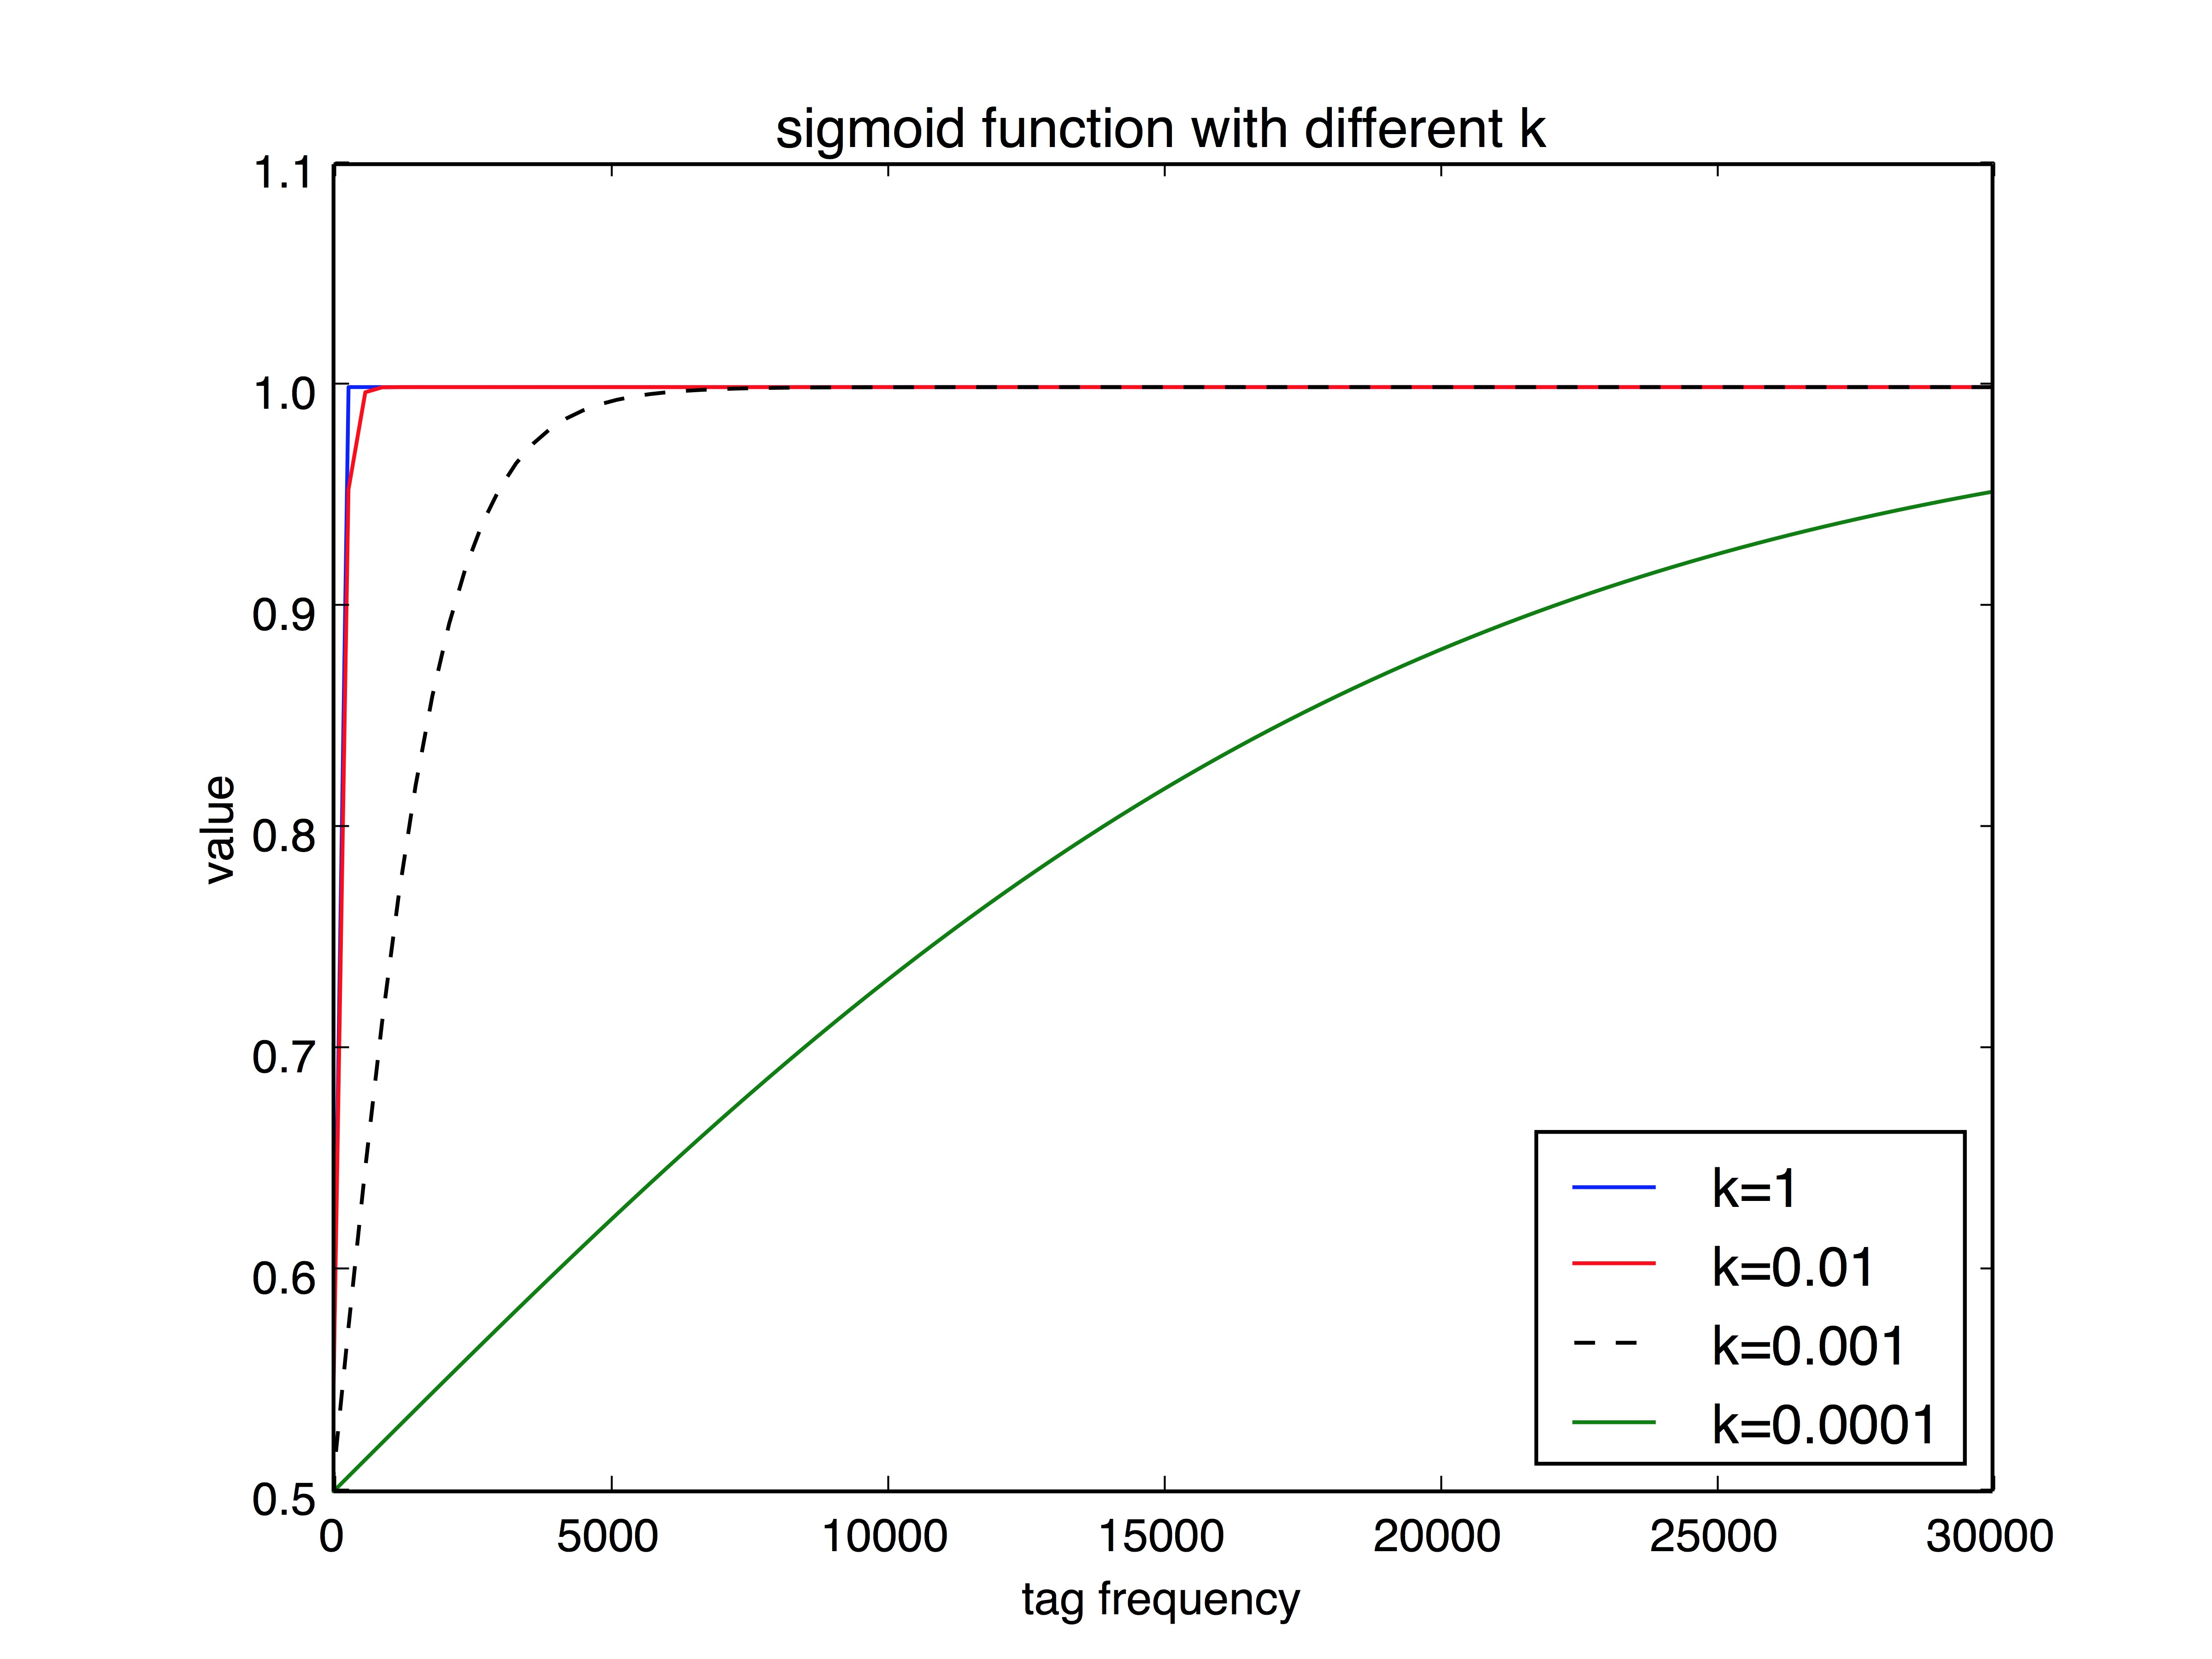
\includegraphics[width=5in]{sigmoid.jpg}  
\caption{Shape of function $\frac{1}{(1+e^{-k*z})}$ for different values of $k$}
\label{fig:sigmoidfunction} 
\end{figure}
For example, if the first-tag frequency map for \textit{css} is \{\textit{html}:10, \textit{jquery}:2\}, then, when normalizing first-tag \textit{html}, $I(T_f,T_i)=10$, $I(T_i)=12$, $I(T_f)=5,552$. As a result, $p(html|css)=0.8301$. 
Similarly, for each tag, we provide a list of candidate first-tags with estimated probabilities. 

The second step of our approach consists in choosing a first-tag to enrich each question. Given a question's tag list, we fetch the top 5 first-tags (with the highest probabilities). Then we accumulate the corresponding probabilities with a discount function taking into account the position of the tag in the tag list associated to the question, as shown in equation \ref{eq:accumulate}: 
\begin{equation}
\begin{split}
 p_{j}=  p_{1,j}+p_{2,j}*dis+...+p_{k,j}*dis^{k-1} \\
\end{split}
\label{eq:accumulate}
\end{equation}

%TODO: you noted there could be two kinds of discount, one is liner discount, another is non-liner, such as log discount. need to prove which is better. 
%DONE
%I put it in the experiment section. 

 %for j \in [1,V], k \in [1,K]
where $p_{j}$ denotes the probability of  tag $j$ to be the first-tag of a given question, $p_{k,j}$ denotes the probability for tag $k$ to have tag $j$ as its first-tag. The range of $v$ and $k$ are $[1,V]$ and $[1,K]$, where $V$ denotes the number of all the first-tags, $K$ denotes the number of tags in the given question and $dis$ denotes the discount due to the position. There are could be two kinds discount function, linear or non-liner (e.g. exponential) discount. We discuss it in experiment section.

Then we consider the first-tag with the highest probability as the enriching first-tag. If this first-tag already exists in the original tag list, we simply skip the insertion, or else we insert it at the first position of the question's tag list. We processed $242,552$ tag lists from the StackOverFlow Q\&A site, and our method enriched $33,622$ of them (13.5\%).

Table \ref{tab:enrichedcompare} presents the results of the enrichment of 8 tag lists (enriched tags are in bold).

\begin{table}[htp]
\caption{Original and enriched tag lists}
\label{tab:enrichedcompare}
\centering
\begin{tabular}{|c|c|}
\hline
ant & \textbf{java}, ant\\
\hline
qt, boost& \textbf{c++}, qt, boost\\
\hline
django, hosting & \textbf{python}, django, hosting \\
\hline
xslt, dynamic, xsl & \textbf{xml}, xslt, dynamic, xsl \\
\hline
sql-server-2005, sorting & \textbf{sql}, sql-server-2005, sorting \\
\hline
tomcat, grails, connection & \textbf{java}, tomcat, grails, connection\\
\hline
cocoa, osx, mac, plugins & \textbf{objective-c}, cocoa, osx, mac, plugins \\
\hline
spring, j2ee, module, count & \textbf{java}, spring, j2ee, module, count \\
\hline
\end{tabular}
\end{table}



\subsection{Efficient topic extraction from tags}
\label{subsec:topicextraction}
From the observation of our dataset, we confirmed the natural intuition that high frequency tags are more generic and low frequency tags are more specific, and most of the low frequency tags are related to a more generic tag. A similar observation was also found in \cite{mika2007ontologies}. Besides, \cite{yang2013cqarank} shows that tag frequency in Q\&A sites also satisfie a power law distribution \cite{adamic2000power}.

For example, for a question tagged with \{\textit{c++,} \textit{iostream,} \textit{fstream}\} (with tags sorted according to their frequencies), we could find that it was related to \textit{c++} and to the \textit{iostream} topic of \textit{c++}, and more specifically, that it focused on \textit{fstream}. This inspired us to build a tag tree to represent it and compute the probability for a tag to be related to a topic. Figure \ref{fig:tagtree} illustrates the process of building a tag tree. Figure \ref{fig:htmltagtree} illustrates an example of \textit{html}'s tree. Our topic extraction method is described in Algorithm \ref{algo:algotopic}. 


\begin{figure}[htp]
\centering
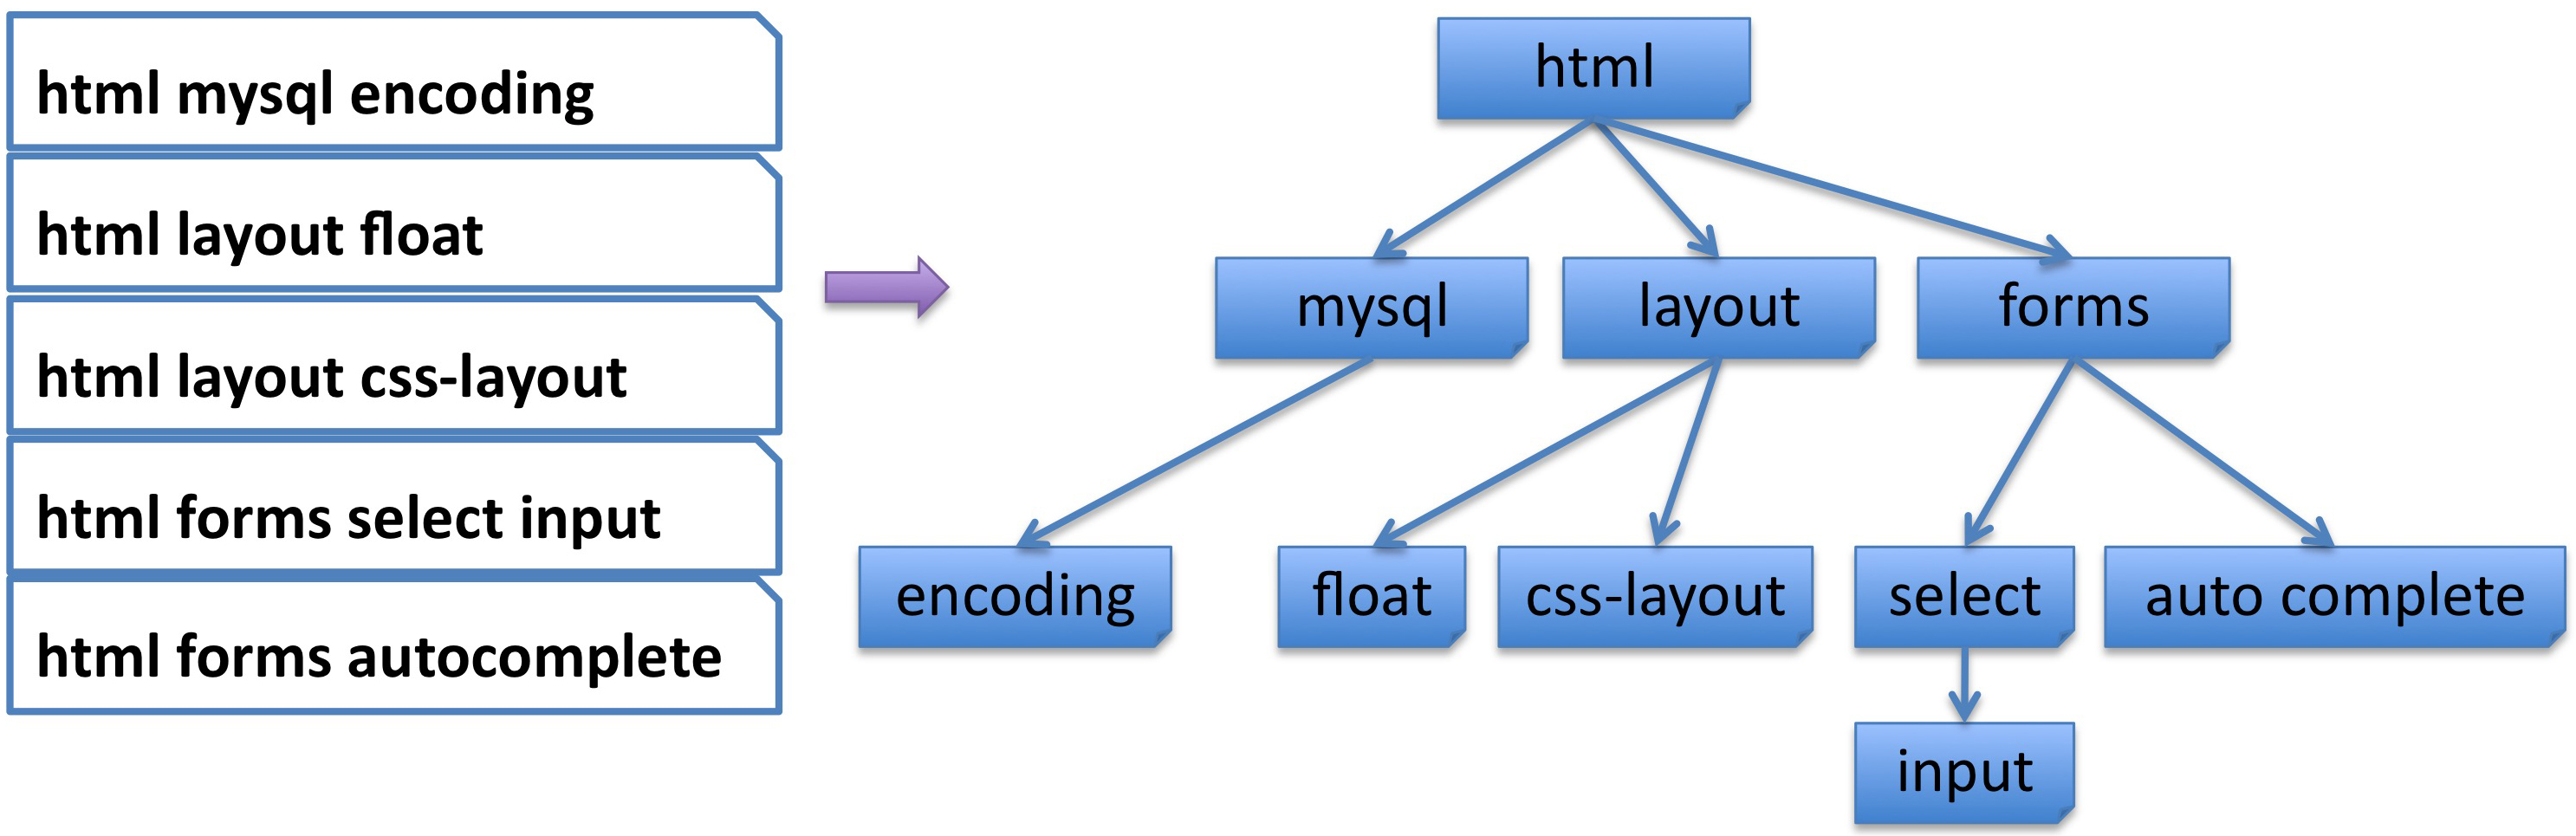
\includegraphics[width=5in]{buildTreeProcess.jpg}  
\caption{Example of a tag tree}
\label{fig:tagtree} 
\end{figure}


%\IncMargin{2em}

\begin{algorithm}%[htp]
\begin{algorithmic}[1]
\label{algo:algotopic}
\State \textbf{Input:} \textit{ enriched tag list of questions, topic number K}
\State \textbf{Output:} \textit{topic-tag distribution}
\State \textit{/*build trees process, shown in Fig \ref{fig:tagtree}*/}

\State trees = null \textit{/* initialize */}
\For { \textit{tag} \textbf{in} \textit{taglist} }%{tag question's taglist}
\State{trees.insert(taglist)}
\EndFor
\State \textit{/*build affinity matrix for root\_tags*/}
\State root\_tags = trees.get\_root\_tags() 
\State   affinities\_matrix = \textbf{build\_affinity}(root\_tags) 
\State  \textit{/*run spectral-clustering on affinity matrix*/}
\State  groups = \textbf{spectral}(\textit{affinities\_matrix,K})
\State  \textit{/*combine tree according to groups*/}
\State  new\_trees = \textbf{combine\_tree} (\textit{trees,groups})   
\State  \textit{/*compute topic-tag distribution*/}
\State  topic\_distributions = \textbf{compute} (\textit{new\_trees})
\State \textit{** we perform a spectral clustering to divide these root tags into several groups}
\end{algorithmic}
\end{algorithm}
%\caption{Topic Extraction}

In the \textit{build trees} process (lines 3-6), we build a tag tree according to the position of tags in a question, and record the occurrence of each node. For example, let us consider again the tag lists of questions Q1, Q2, Q3 in Figure~\ref{fig:examplefirsttag}. Based on them, we construct two trees. The root of the first tree is \textit{html}, the occurrence of this node is \textit{2}, it has only one child \textit{css}, which has \textit{2} occurrences, and this node has two children, \textit{layout} and \textit{height}, and each one occurs \textit{1} time. The root of the second tree is \textit{c\#} with \textit{1} occurrence.

By processing all the tag lists, many trees are generated. We then construct an affinity matrix of the root nodes (lines 7-9). Since we applied our first-tag enrichment method, the number of root tags is not very large. The similarity of two root nodes is computed according to equation \ref{eq:simi}:


\begin{equation}
Simi(R_i,R_j)= \frac{I(R_i,R_j)}{(I(R_i)+I(R_j))}
\label{eq:simi}
\end{equation}

where $I(R_i,R_j)$ denotes the co-occurrence of root tag $R_i$ and root tag $R_j$, and $I(R_i)$ and $I(R_j)$ denote the occurrence of root tag $R_i$ and root tag $R_j$ respectively. Then we perform a spectral clustering~\cite{Ng01onspectral} on the affinity matrix to group these root nodes  (line 10-11). Each group forms what we will call a topic. As spectral clustering requires to select the desired number of topics, we choose the same number \textit{30} as~\cite{Chang:2013}, which has proved to be a reasonable setting for the Stackoverflow dataset.

We then combine trees if their root nodes belong to the same topic (lines 12-13). This process leads to a forest where each tree represents a topic. Then, in the \textit{compute topic-tag distribution} process (lines 14-15), for each topic tree, we compute $p(t|k)$, which denotes the probability of tag $t$ belong to topic $k$, by using the Maximum Likelihood estimation (MLE), according to equation \ref{eq:laplace}: 
%TODO: MLE as not been explained, referenced of even expended in the text above.
%DONE

\begin{equation}
%\begin{split}
p(t|k) = \frac{p(t,k)}{p(k)} = \frac{I(t)+1}{\sum I(t)+N}
\label{eq:laplace}
%\end{split}
\end{equation}

%\begin{equation}
%p(tag|topic)= \frac{p(tag,topic)}{p(topic)} = \frac{I(tag)}{I(sum(tag))}
%\label{eq:computesub}
%\end{equation}

where $I(t)$ denotes the number of occurrences of tag $t$ in the topic tree $k$, and $\sum I(t)$ denotes the total number of occurrences of all tag occurrences in the topic tree.

\begin{figure}[!htp]
\centering
%\epsfig{file=fly.eps, height=1in, width=1in} % use this if you use "pdflatex"
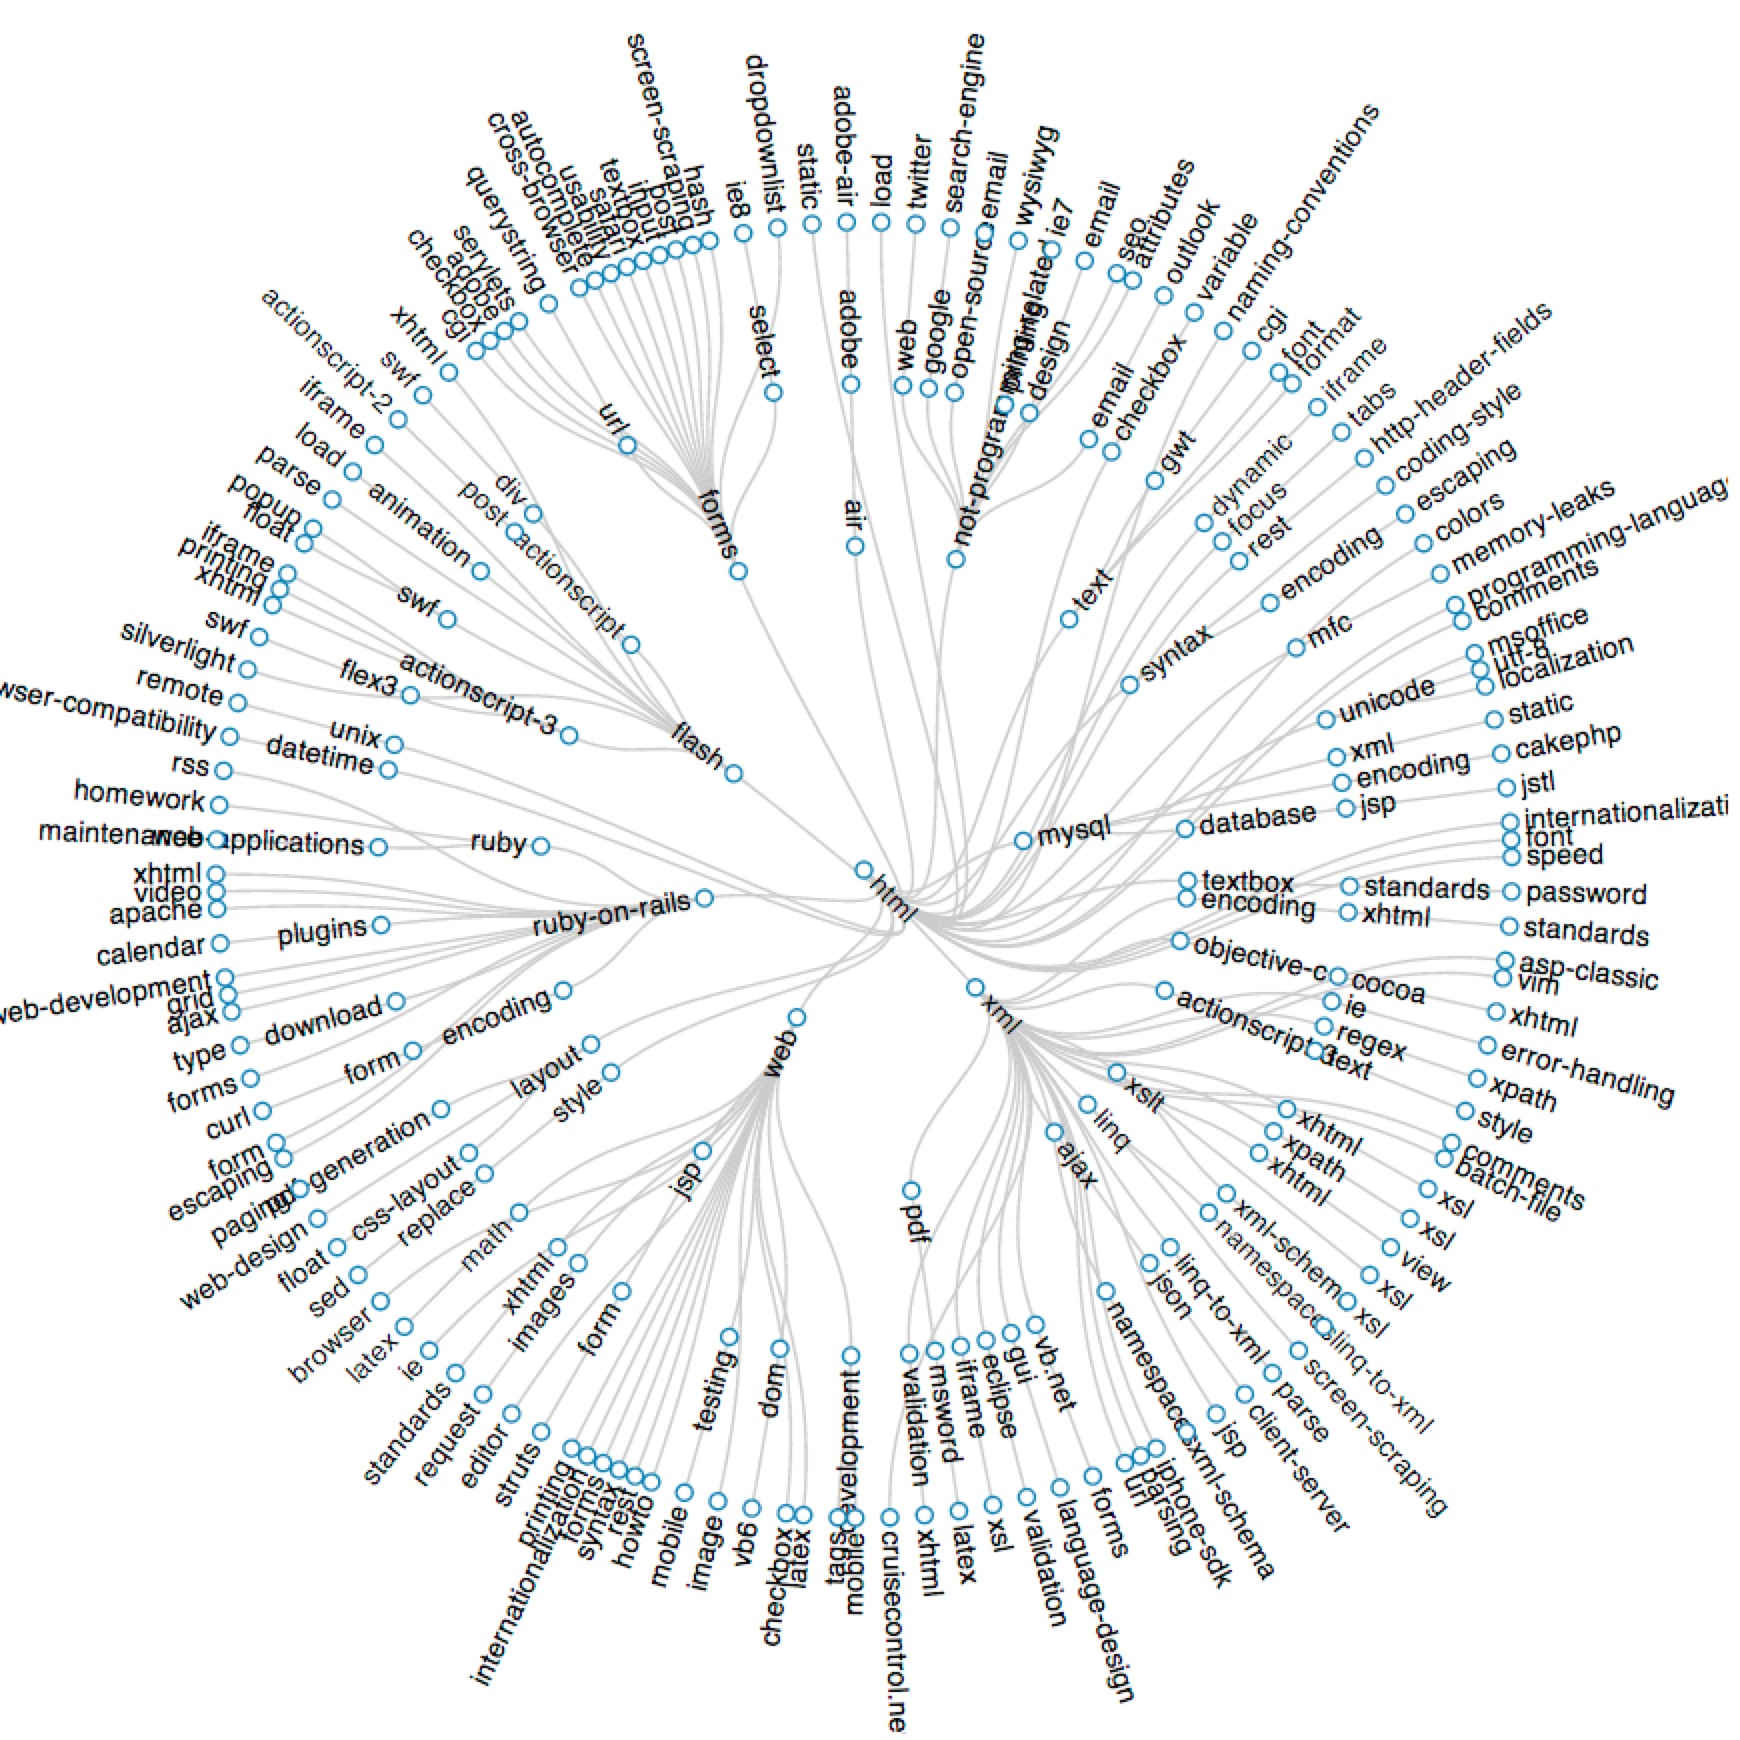
\includegraphics[width=5in]{tag_prefixtree.png}  
\caption{\textit{html}'s tag tree}
\label{fig:htmltagtree} 
\end{figure}

%$p$ and $I(p)$ respectively denote the probability and the number of occurrences of a parent tag, $p\_sub\_i$ and $I(sub\_i)$ denote the probability and the number of occurrences of the $i-th$ child tag. We estimate the probability of $p\_sub\_i$ by equation \ref{eq:computesub},
%\begin{small}
%\end{small}
%p\_sub\_i=\frac{I(sub_i)}{I(p)} * p

Compared with LDA-based model, our model could have a zero-probabilities problem, with less popular or new tags related to some topics with a zero probability due to no evidence of co-occurrence. For example, if tag \textit{zombie-process} never occurs in a \textit{html}-related tag tree, then the probability of tag \textit{zombie-process} to be related to \textit{html-related} topics is zero, which could lead to some problems when dealing with young datasets. We avoid it by using the Laplace smoothing method, as shown in equation \ref{eq:laplace}. Table \ref{tab:toptagspttd} shows the top tags and their probabilities detected by our method.

% TODO: integrate proof here, in this paper that says LDA needs hundreds of iterations to find stable results.\cite{griffiths2004finding}
%DONE
In addition, compared with LDA-based model, our model is much simpler and faster. The probabilistic graphical model requires hundreds of iterations to get stable results~\cite{griffiths2004finding}.

We used the spectral clustering implementation of scikit-learn toolkit\footnote{Scikit-learn toolkit: \\ \indent \url{http://scikit-learn.org/stable/modules/clustering.html#spectral-clustering}}. We only run it on the set of root nodes, which has quite a small size (around 1175 nodes after the tag enrichment process), which means that we only need to build an affinity matrix on these root nodes and the overall cost therefor remains acceptable.

\subsection{User Interest Detection: assigning users to topics}
\label{sec:uidetect}
In StackOverflow, users answering a question can be considered as interested in the topics denoted by the tags of the question. As a result, a starting point for user interest detection is to model the initial situation as follows: a user answering a question acquires the tags attached to this question and gradually, each user acquires a list of tags.

So we represent a user by a tag list: $U= \{U_i | i=1,...,n\},U_i=\{tag_i|i=m,n,...,k\}$, and our goal is, for each user $U_i$, to find $I_i=\{I_{i1},I_{i2}...I_{ik}\}$ where $I_{ik}$ denotes the probability of user $U_i$ to be related to $topic_k$. As we already have a topic-tag distribution %(see section \ref{subsec:topicextraction})
we simply compute the user-topic distribution according to equation \ref{eq:getuserinterest} where $P_{t,k}$ denotes the probability of tag $t$ to be related to topic $k$. We then normalize the probabilities between 0 and 1 by dividing the global max value. We use the $log$ function for numerical stability. Here we do not apply normalization at the level of the user, because like \cite{yang2013community}, we believe that each user could have a high interest in two or more topics simultaneously, while most of the probabilistic graphical models including LDA and PLSA require that the sum of all the probabilities is 1, which means that a user cannot have high probabilities to many topics simultaneously. Our method does not have this limitation. 

Then we identify users' communities of interests based on the user-topic distribution: a user having a high probability for a topic should be a member of the community represented by this topic.

\begin{equation}
 I_{i,k} = log \left\{\sum_{t=1}^{v} P_{t,k}  +1 \right\}\\
  %\begin{cases}
  %* :\text{if } tag_t \in U_i
  %\end{cases}
\label{eq:getuserinterest}
\end{equation}
%0       & \text{if } tag_t \notin U_i \\




\section{TTD Experiments and Evaluation on StackOverflow data}\label{sec:TTDexperiment} 
We conducted experiments on the dataset of activities on StackOverflow between 2008 and 2009, which is available online\footnote{\url{https://archive.org/details/stackexchange}}, to evaluate the performance of our TTD approach compared to three other community detection algorithms. 
%\subsection{Dataset Description}
Some basic statistics of the dataset are given in Table \ref{tab:stackoverflowdataset}. We see that the total number of users arround 100K and among them, 47K users submitted at least one question, and 54K users answered at least one question. The total number of tags attached to questions is 24K, and 20\% of them are used more than 10 times. The frequency of tags follows a power law distribution. The total number of posts is 1.1M; among them there are 242K questions and 870K answers. If two users answer the same question, then the two users are wired by a co-answer link. We filtered the co-answer links with a rule stating that a link is kept if two users answer the same questions more than 10 and 20 times. As a result, we obtained two noise-less datasets. 

% TODO: I uncommented the table and referenced it from the text please check it.
%DONE

\begin{table}[htp]
\caption{Basic statistics of the stackoverflow dataset}
\label{tab:stackoverflowdataset}
\centering
\begin{tabular}{|c|c|c|c|c|}
\hline
\textbf{item} & \textbf{description} \\
\hline
total users & 103K (47K questioner, 54K answerer)\\
\hline
total tags & 24K (20\% used more than 10 times)\\
\hline
total posts & 1.1M (question 242K, answer 870K) \\
\hline
co\_answer\_10 & 902 users, 6746 co\_answer link\\
\hline
co\_answer\_15 & 401 users, 2326 co\_answer link\\
\hline
co\_answer\_20 & 241 users, 1064 co\_answer link\\
\hline
co\_answer\_25 & 153 users, 592 co\_answer link\\
\hline
labeled user & 902 users, 1$\sim$3 labels per user\\
\hline
\end{tabular}
\end{table}

% TODO: I uncommented the figures but they need to be checked and commented in the text. 
%DONE

% TODO: include all the figures, charts, graphics, etc. you have, add a label and caption and comment them in the text
%DONE

%new version of this image is in discusstion section.
%
%\begin{figure}[htp]\centering
%\epsfig{file=fly.eps, height=1in, width=1in}
%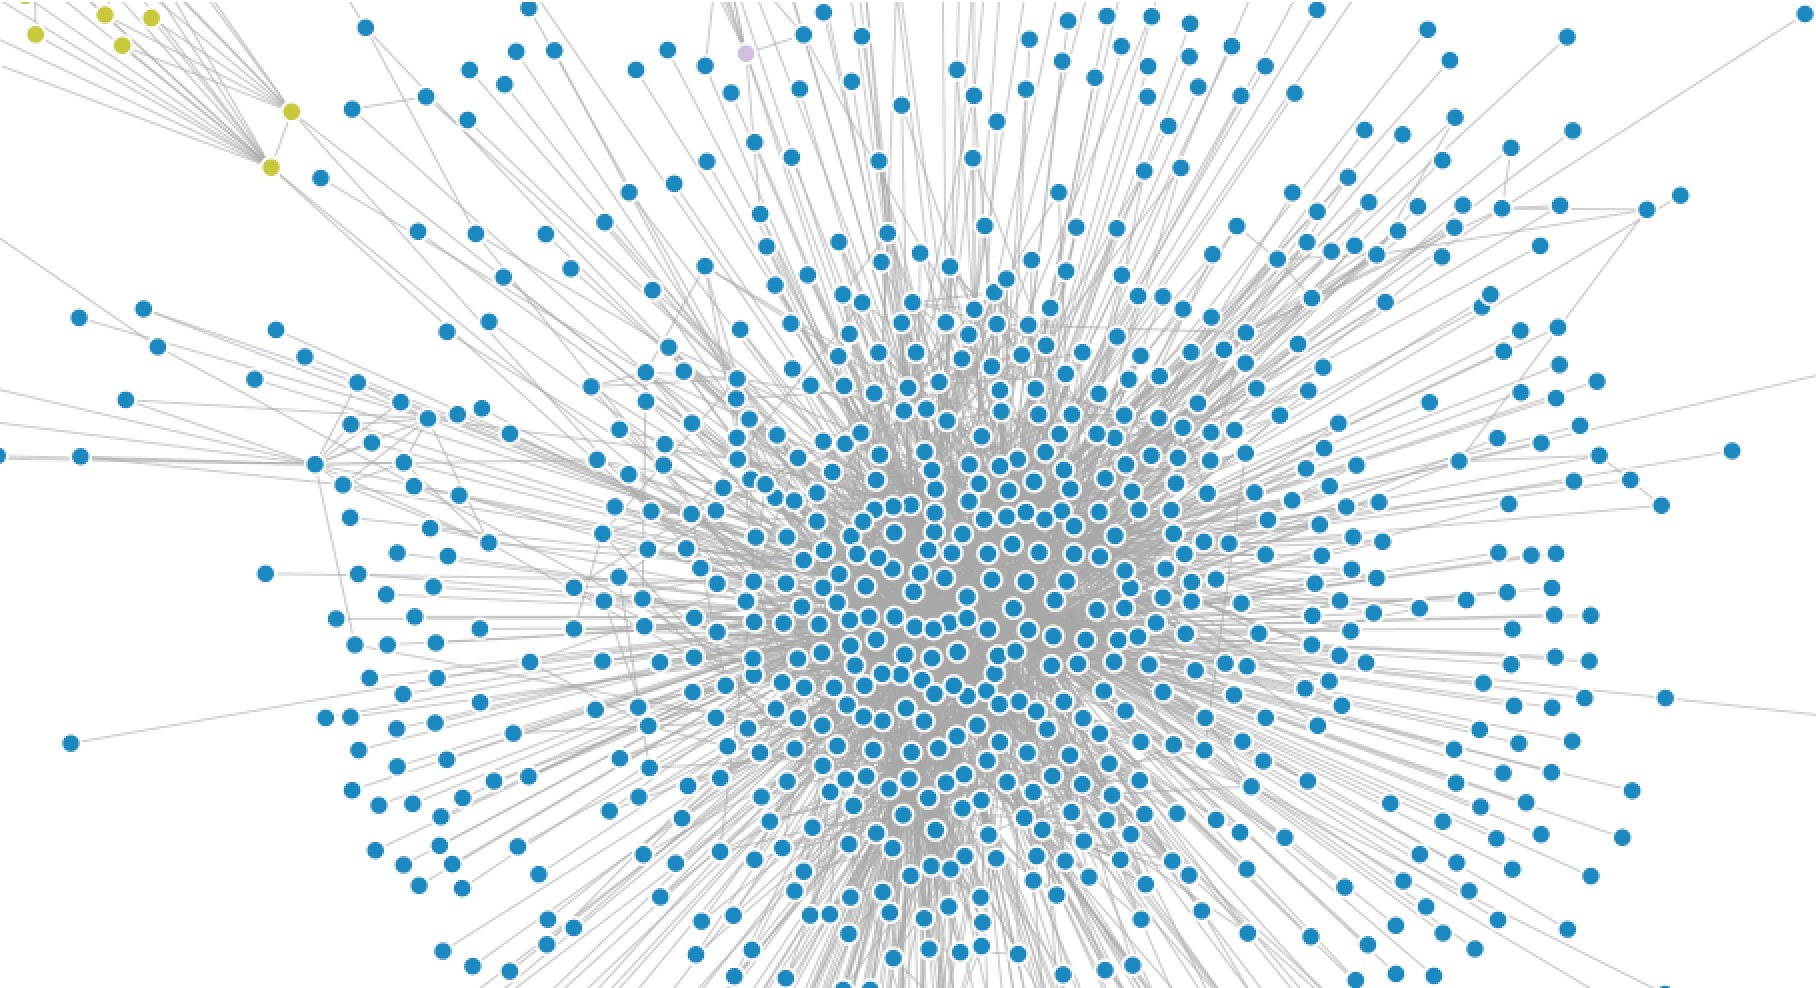
\includegraphics[width=5in]{lpa_co_answer_10.png}  % use this if you use "pdflatex"
%\caption{\# of user answered and asked question}
%\label{fig:qaheatmap} % Fig.2
%\end{figure}

% TODO: why is the following text here ? duplicate with last section ?
%DONE
% i comment this part because dont use user study section.
%Then we manually labeled the 'co\_answer\_10' 902 users to evaluate the results obtained on the four datasets by comparing them with our manual labelling.
%\subsection{Evaluations}
%\vspace{-2em}

\subsection{Performance of Topic Extraction: perplexity metric}
We use the Perplexity~\cite{blei2003latent} metric to measure the topic extraction performance. It is a common metric in the topic modeling area, measuring how well the words in test documents are represented by the word distribution of extracted topics. The intuition is that a better model will tend to assign higher probabilities to the test dataset, corresponding to a lower perplexity value. We split the dataset (question tag lists), 80\% as training set, 20\% as testing set.
% TODO: do we need to to a k-fold cross validation or not?
% TBD
We run LDA and our method on the training set to get the topic distribution. Then for a test set of M questions' tag lists ($N_d$ denotes the number of tags in the $d^{th}$ question) the Perplexity score is computed as shown in equation \ref{eq:gettagperplexity}:
%\begin{small}
\begin{equation}
  Perplexity(D_{test})=exp\left\{-\frac{\sum_{d=1}^{M}\log p(t)}{\sum_{d=1}^{M}N_d}\right\}
\label{eq:gettagperplexity}
\end{equation}

\begin{figure}[htp]
\centering
%\epsfig{file=fly.eps, height=1in, width=1in}
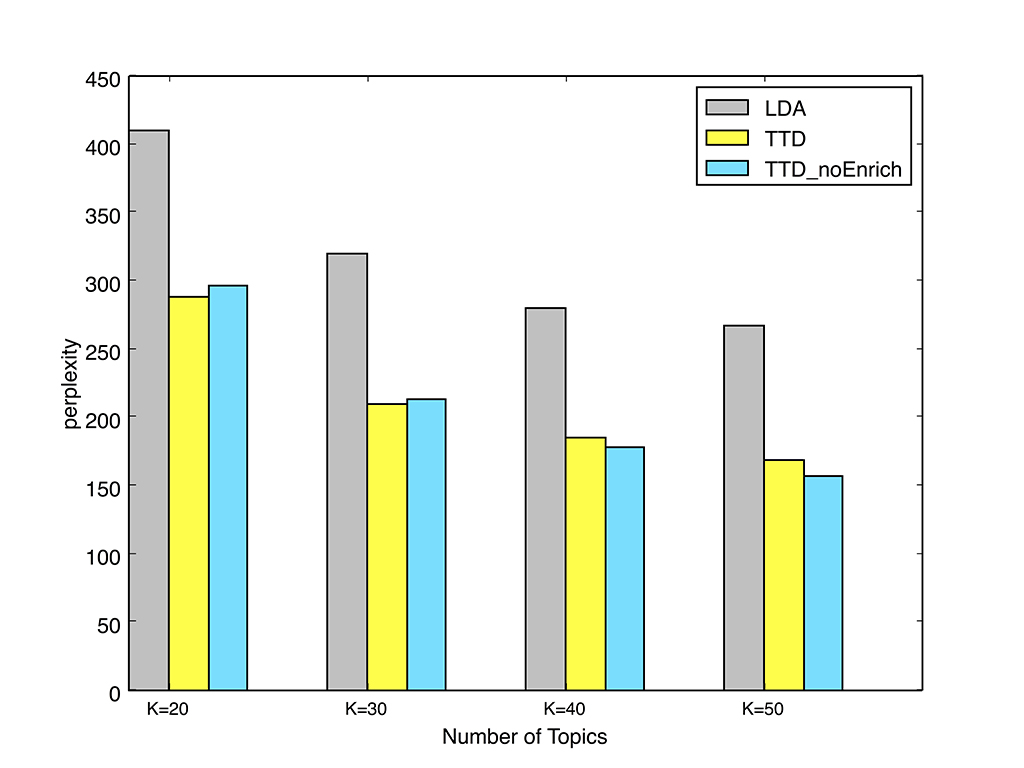
\includegraphics[width=5in]{perplexity.jpg}  % use this if you use "pdflatex"
\caption{Comparison of topic extraction performances}
\label{fig:tagperplexity} 
\end{figure}

In our model, $p(t)$ is equal to $p(k|q)*p(t|k)$. We compute the topic-question distribution $p(k|q)$ similarly to the user-topic distribution (see Section \ref{sec:uidetect}), by replacing user's tag lists by question's tag lists. The only difference is that we normalize the question-topic distribution to make sure that the sum of a question's topic distribution is 1. We show and compare the average perplexity score in Figure \ref{fig:tagperplexity}. \textit{TTD} is our method, \textit{TTD\_noEnrich} represents our method without first-tag enrichment. We find that TTD could outperform the state-of-the-art LDA method. The reason is that, compared with traditional document topic modeling use cases, question tag lists in Q\&A sites are very short, and LDA performs poorly in this situation. Besides, our first-tag enrichment method can improve the performance when the number of topics is not very large. 

We use different discount functions, which is used in equation \ref{eq:accumulate}, and compare the perplexity score. we found that the performance of using discount is better than not using discount. And the liner discount is better than exponential discount. 
% 1 0.8 0.6 0.4 0.2:    212  liner
% 1 0.5 0.25 0.125 :    213  exponential
% 1 1 1 1 1        :    215  not using

Another point is that, benefiting from a tree structure for topics, we can easily extract sub-topics from a given topic. Besides, TTD is based on a topic model, so extracting these sub-topics can help us find sub-communities within a detected community. Table \ref{tab:comparedwithsubtopic} shows the top tags of \textit{java}'s sub-topic \textit{html} and of topic \textit{html}. We can find that the differences are noticeable for topics: a user who is interested in topic \textit{html} is not necessarily interested in \textit{java}'s sub-topic \textit{html} and vice versa. 

\begin{table}[htp]
%\begin{table}[!t]
\caption{Top tags and their probabilities for some topics computed with TTD}
\label{tab:toptagspttd}
\centering
%\scriptsize
%\begin{tabular}{|p{37pt}|p{10pt}|p{31pt}|p{10pt}|p{43pt}|p{10pt}|}
\begin{tabular}{|c|c|c|c|c|c|}

\hline
\multicolumn{2}{|c|}{topic4} & \multicolumn{2}{c|}{topic5} & \multicolumn{2}{c|}{topic6}  \\
\hline
iphone&0.203&git&0.198&sql&0.177\\
\hline
objective-c&0.112&svn&0.096&mysql&0.122\\
\hline
ios&0.109&version-control&0.045&sql-server&0.074\\
\hline
xcode&0.042&github&0.033&database&0.040\\
\hline
cocoa-touch&0.021&tfs&0.033&oracle&0.030\\
\hline
ipad&0.020&maven&0.029&sql-server-2008&0.029\\
\hline
cocoa&0.018&tortoisesvn&0.018&tsql&0.026\\
\hline
uitableview&0.012&msbuild&0.016&query&0.025\\
\hline
ios5&0.010&jenkins&0.015&sql-server-2005&0.019\\
\hline
core-data&0.009&tfs2010&0.014&database-design&0.011\\
\hline
\hline
\multicolumn{2}{|c|}{topic12} & \multicolumn{2}{c|}{topic13} & \multicolumn{2}{c|}{topic14}   \\
\hline
html&0.214&javascript&0.264&machine-learning&0.247\\
\hline
css&0.201&jquery&0.114&artificial-intelligence&0.130\\
\hline
xhtml&0.017&html&0.035&neural-network&0.062\\
\hline
web-development&0.016&ajax&0.031&classification&0.046\\
\hline
ie&0.012&css&0.016&data-mining&0.037\\
\hline
css-layout&0.010&firefox&0.013&svm&0.031\\
\hline
div&0.010&dom&0.011&weka&0.025\\
\hline
layout&0.010&php&0.011&libsvm&0.015\\
\hline
firefox&0.009&ie&0.010&nlp&0.024\\
\hline
ie6&0.009&web-development&0.008&bayesian&0.011\\
\hline
\end{tabular}
\end{table}

\begin{table}[htp]
\caption{Top tags for \textit{java}'s sub-topic \textit{html} and \textit{mysql}, denoted by java\_html, and java\_mysql respectively, compared with topics \textit{html} and \textit{mysql}}
\label{tab:comparedwithsubtopic}
\centering
%\tiny
\begin{tabular}{|p{0.8in}|p{4.2in}|}
%\begin{tabular}{|c|l|}
\hline
java\_html& jsp swing xml parsing jsf jeditorpane pdf applet dom\\
\hline
html & css xhtml web-development table div ie layout css-layout firefox\\
\hline
\hline
java\_mysql&jdbc hibernate database tomcat prepared-statement spring connection-pooling connection security \\
\hline
mysql &database query mysql-query ruby-on-rails database-design performance stored-procedures innodb optimization\\
\hline
\end{tabular}
\end{table}

\subsection{Performance of User Interest Detection: Similarity metrics}
Traditional community detection algorithms are based on a network structure. As there is no explicit network in our dataset and in order to compare our work with other approaches on the same dataset, we extracted a network of interactions between users: a co-answer network inspired by the notion of co-view network introduced in~\cite{DBLP:conf/icwsm/GargiLMY11}. The idea behind it is that if two users answer the same question they share some of their interests. So, the co-answer network, to some extent, can reflect the common interests between users. We filtered the co-answer links with a rule stating that a link is kept if two users answer the same questions more than 10 times and 20 times.
% TODO: in a PhD thesis there is no size constraint so you should give all your experiments 10 to 25
%DONE, add 20.

Based on the noise-less dataset obtained, we implemented three well known community detection methods in order to compare our approach with them.

In order to evaluate the results of overlapping community detection, for each user, a method should output $1\sim3$ community labels with corresponding probabilities to indicate to what extent the user is interested in the community. Then we define three levels of interest in a community: \textit{High}, \textit{Medium}, \textit{Low} according to the probabilities. In addition, we empirically set the number of communities to $30$ for all the evaluated methods.
\begin{itemize}
\item{SLPA~\cite{DBLP:journals/csur/XieKS13}}: An overlapping community detection method inspired by a classical Label propagation algorithm (LPA). SLPA algorithm can evaluate to which extent a user belongs to a community by the received propagated label (a 'Post-process' in SLPA algorithm). So, it can output more than one community label according to these frequencies.
\item{LDA}: Similar to~\cite{yang2013cqarank}, we run LDA to build a user-topic-tag model on the given dataset, users are represented by their tag list. As the output contains a user-topic distribution, we just sort the distribution for each user and choose the top 3 topic labels as community label together with their probabilities.
\item{Clustering}: We used the implementation of hierarchical clustering from scikit-learn toolkit\footnote{\url{http://scikit-learn.org/stable/modules/clustering.html#hierarchical-clustering}}. As clustering algorithms are hard-partitioned, it can only generate one group label for each user.
\item{TTD}: it is our method. We sort the results of user interest detection (section \ref{sec:uidetect}) and choose the top 3 as community label together with their probabilities.
\end{itemize}

% TODO: you noted that "this part still need to improve..... to do work."
% forgot it...

Our aim was to evaluate the similarity between users within a detected community of interest. We mainly used the \textit{jaccard similarity} and \textit{cosine similarity} of two user's tag lists to evaluate the similarity of two user's interests. We used a modified modularity metric to compute the difference between the average similarity between the users within a community ($avg\_inner$) and the average similarity between the users in a community and some user randomly chosen from the whole dataset ($avg\_rand$). This is captured in Equation \ref{eq:nmi}, where $N$ represents the number of users in a community $C$, and $Simi$ denotes the similarity function. $Rand\_U$ represents users that are randomly chosen from the whole data set. A higher value of $avg\_inner$ denotes that users within a community are very similar. A lower value of $avg\_rand$ denotes that users of a community are not very similar to random users. So a higher value of $modularity$ means a larger difference between $avg\_inner$ and $avg\_rand$, which is considered as a better partition of communities. As the metric has random variables, we run the experiments 10 times and each time we used different random users. Besides, we created a \textit{center} user in each community by averaging all users' tag lists and frequencies, then we computed the average similarity between each user in a community and this \textit{center} user as $avg\_center$. 
As introduced before, each method gives $1\sim3$ community labels for each user to indicate the level of interest. So we evaluated each level of interest respectively.

\begin{equation}
%\tiny
%\begin{split}
  M(C) \\
  =\frac{Avg\_inner(\sum_{i=1}^{N}\sum_{j=1}^{N} Simi(U\_i,U\_j))}{Avg\_rand(\sum_{i=1}^{N}\sum_{j=1}^{50} Simi(U\_i,Rand_U\_j))}
\label{eq:nmi}
%\end{split}
\end{equation}

Experiment results are shown in Table \ref{tab:uidcompare10} and \ref{tab:uidcompare20}. We run each method on the co-answer-10 and co-answer-20 dataset 10 times, and listed the average value. We found that our method is better than the three other methods in detecting users' \textit{High} level of interest with both metrics. The reason why our method is not very efficient to detect users' \textit{Low} level of interest is that our method allows users to belong to more than one community with high probabilities, since our method do not have the sum-to-one constrain. For example, a user could be interested in a topic with a probability of 0.7 (High) and interested in several topics with a probability of 0.3 (Low), where the sum of these probabilities not equal to 1. Then this user will be in many \textit{Low} level of interest communities. This puts some irrelevant users with \textit{Low} level of interest which decreases the similarity between community members.




\begin{sidewaystable}

%\begin{table*}[htp]
\caption{Comparison of the performances of the methods of user interest detection on co\_answer\_10 dataset}
\label{tab:uidcompare10}
%\tiny
\scriptsize
\centering
%\begin{tabular}{|p{60pt}||p{60pt}||p{60pt}|}
%\begin{tabular}{|p{23pt}|p{23pt}|p{23pt}|p{23pt}|p{23pt}|p{23pt}|p{23pt}|p{23pt}|p{23pt}|p{23pt}|p{23pt}|p{23pt}|p{23pt}|}
\begin{tabular}{|c|c|c|c|c|c|c|c|c|c|c|c|c|}

\hline
Similarity & \multicolumn{12}{c|}{Jaccard Similarity}  \\
\hline
Level  &  \multicolumn{4}{c|}{High Interest} & \multicolumn{4}{c|}{Medium Interest} &  \multicolumn{4}{c|}{Low Interest} \\
\hline
Metric  & avg\_inner & avg\_rand & \textit{modularity} & avg\_center& avg\_inner & avg\_rand & \textit{modularity} & avg\_center& avg\_inner & avg\_rand & \textit{modularity} & avg\_center \\
\hline
TTD&\textbf{0.162}&\textbf{0.033}&\textbf{4.909}&\textbf{0.218}&\textbf{0.135}&\textbf{0.039}&\textbf{3.462}&0.171&0.107&0.042&2.548&0.131\\
\hline
LDA&0.147&0.035&4.200&0.178&0.131&0.039&3.359&\textbf{0.177}&\textbf{0.144}&0.041&\textbf{3.512}&\textbf{0.193}\\
\hline
SLPA&0.131&0.040&3.275&0.166&0.129&0.040&3.225&0.159&0.121&\textbf{0.039}&3.103&0.155\\
\hline
Clustering&0.130&0.041&3.171&0.161&0.000&0.000&0.000&0.000&0.000&0.000&0.000&0.000\\
\hline
Similarity & \multicolumn{12}{c|}{Cosine Similarity}  \\
\hline
Level  &  \multicolumn{4}{c|}{High Interest} & \multicolumn{4}{c|}{Medium Interest} &  \multicolumn{4}{c|}{Low Interest} \\
\hline
Metric  & avg\_inner & avg\_rand & \textit{modularity} & avg\_center& avg\_inner & avg\_rand & \textit{modularity} & avg\_center& avg\_inner & avg\_rand & \textit{modularity} & avg\_center \\ 
\hline
TTD&0.736&\textbf{0.574}&\textbf{1.282}&0.857&0.573&\textbf{0.602}&0.952&0.761&0.475&0.629&0.755&0.695\\ \hline
LDA&\textbf{0.836}&0.660&1.267&\textbf{0.917}&\textbf{0.900}&0.612&\textbf{1.471}&\textbf{0.948}&\textbf{0.757}&\textbf{0.600}&\textbf{1.262}&\textbf{0.865}\\ \hline
SLPA&0.749&0.624&1.200&0.854&0.590&0.621&0.950&0.687&0.702&0.625&1.123&0.844\\ \hline
Clustering&0.763&0.622&1.226&0.875&0.000&0.000&0.000&0.000&0.000&0.000&0.000&0.000\\ \hline
\end{tabular}
%\end{table*}

\end{sidewaystable}




\begin{sidewaystable}

%\begin{table*}[htp]
\caption{Comparison of the performances of the methods of user interest detection  on co\_answer\_20 dataset}
\label{tab:uidcompare20}
%\tiny
\scriptsize
\centering
%\begin{tabular}{|p{60pt}||p{60pt}||p{60pt}|}
%\begin{tabular}{|p{23pt}|p{23pt}|p{23pt}|p{23pt}|p{23pt}|p{23pt}|p{23pt}|p{23pt}|p{23pt}|p{23pt}|p{23pt}|p{23pt}|p{23pt}|}
\begin{tabular}{|c|c|c|c|c|c|c|c|c|c|c|c|c|}

\hline
Similarity & \multicolumn{12}{c|}{Jaccard Similarity}  \\
\hline
Level  &  \multicolumn{4}{c|}{High Interest} & \multicolumn{4}{c|}{Medium Interest} &  \multicolumn{4}{c|}{Low Interest} \\
\hline
Metric  & avg\_inner & avg\_rand & \textit{modularity} & avg\_center& avg\_inner & avg\_rand & \textit{modularity} & avg\_center& avg\_inner & avg\_rand & \textit{modularity} & avg\_center \\
\hline
TTD&\textbf{0.175}&0.034&5.121&\textbf{0.232}&\textbf{0.153}&0.038&4.025&\textbf{0.189}&0.115&0.043&2.695&0.132\\
\hline
LDA&0.160&\textbf{0.028}&\textbf{5.742}&0.198&0.139&0.030&\textbf{4.623}&0.188&\textbf{0.174}&0.037&\textbf{4.697}&\textbf{0.224}\\
\hline
SLPA&0.126&0.029&4.290&0.167&0.057&\textbf{0.014}&4.104&0.078&0.064&\textbf{0.015}&4.394&0.087\\
\hline
Clustering&0.164&0.038&4.303&0.206&0.000&0.000&0.000&0.000&0.000&0.000&0.000&0.000\\
\hline
Similarity & \multicolumn{12}{c|}{Cosine Similarity}  \\
\hline
Level  &  \multicolumn{4}{c|}{High Interest} & \multicolumn{4}{c|}{Medium Interest} &  \multicolumn{4}{c|}{Low Interest} \\
\hline
Metric  & avg\_inner & avg\_rand & \textit{modularity} & avg\_center& avg\_inner & avg\_rand & \textit{modularity} & avg\_center& avg\_inner & avg\_rand & \textit{modularity} & avg\_center \\ 
\hline
TTD&0.676&\textbf{0.594}&1.138&0.818&0.548&0.621&0.883&0.745&0.471&0.644&0.730&0.690\\ \hline
LDA&\textbf{0.858}&0.627&\textbf{1.367}&\textbf{0.926}&\textbf{0.888}&\textbf{0.608}&\textbf{1.462}&\textbf{0.939}&\textbf{0.755}&\textbf{0.610}&\textbf{1.237}&\textbf{0.865}\\ \hline
SLPA&0.729&0.632&1.152&0.845&0.695&0.630&1.104&0.834&0.679&0.632&1.074&0.826\\ \hline
Clustering&0.762&0.627&1.216&0.875&0.000&0.000&0.000&0.000&0.000&0.000&0.000&0.000\\ \hline
\end{tabular}
%\end{table*}

\end{sidewaystable}






Table \ref{tab:ourmodelresult} shows some users and their interests detected with TTD and their top 10 tags. The first row contains user ids, the second row contains their detected communities of interests with their probabilities. The following ten rows show the top 10 tags for each user. We replaced community labels by names assigned according to the tags associated to each topic of interest.


\begin{sidewaystable}

%\begin{table}[htp]
\caption{Examples of user interests detected with TTD}
\label{tab:ourmodelresult}
%\scriptsize
\centering
%\begin{tabular}{|p{60pt}|p{60pt}|p{60pt}|}
\begin{tabular}{|c||c||c|}
\hline
user\_10224&user\_103043&user\_113570\\
\hline
database (0.805)\newline c\#-dev (0.081)&java-dev (0.664)\newline database (0.105)&c\#-dev (0.393)\newline web-dev (0.328)\\
\hline
sql-server (21)&java (135)&c\# (107)\\
%\hline
sql (21)&swing (28)&jquery (89)\\
%\hline
tsql (6)&oracle (27)&javascript (56)\\
%\hline
performance (4)&sql (23)&.net (47)\\
%\hline
database (4)&subjective (15)&asp.net (27)\\
%\hline
stored-procedures (3)&windows (13)&css (23)\\
%\hline
sql-server-2005 (3)&eclipse (12)&regex (20)\\
%\hline
.net (3)&best-practices (12)&html (20)\\
%\hline
mysql (2)&plsql (10)&iphone (12)\\
%
sql-server-2000 (2)&regex (10)&string (10)\\
\hline
user\_24181&user\_34509&user\_30461\\
\hline
web-dev (0.743), database (0.072)&c-dev (0.663), linux-dev (0.083)&ios-dev (0.885), linux-dev (0.020)\\
\hline
php (304)&c++ (703)&cocoa (333)\\
%\hline
javascript (193)&c (187)&objective-c (184)\\
%\hline
mysql (116)&templates (62)&iphone (47)\\
%\hline
html (86)&stl (53)&cocoa-touch (39)\\
%\hline
css (57)&linux (48)&osx (35)\\
%\hline
regex (40)&subjective (45)&mac (34)\\
%\hline
jquery (37)&pointers (44)&iphone-sdk (20)\\%
%\hline
sql (27)&java (42)&xcode (18)\\
%\hline
ajax (26)&bash (40)&cocoa-bindings (18)\\
%\hline
apache (23)&boost (31)&core-graphics (18)\\
\hline
\end{tabular}
%\end{table}


\end{sidewaystable}




%TODO: why is the following text commented ?
%DONE  I think it may cause bias because of the human judgement since it's complained by many reviewers

\subsection{User Study: ranking users' interested topics}
In order to evaluate the quality of whether a user is correctly assigned to the right interest group, and to which extent the user belongs to the interest group. To achieve this, we conducted a user survery on the dataset by inviting 2 volunteers as annotators. We asked a volunteer to manually label 902 users (refer to the co\_answer\_10 dataset) by assigning each user up to 3 labels out of eight group labels, chosen from \textit{c-development} group, \textit{java-development} group, \textit{c\#-development} group, \textit{web-development} group, \textit{ios-development} group, \textit{database} group, \textit{linux-development} group and \textit{other-topic} group. 
For example, if user A sequentially has three group labels, \textit{java-development},\textit{web-development},\textit{ios-development}, it means that user A has a big interest in the group \textit{java-development}, a medium interest in the group \textit{web-development}, a lower interest in the group \textit{ios-development}. Since each user has an ordered label list, we have to evaluate both the correctness of detected groups and the correctness of the order. 
We ask another volunteer (who was not involved in labeling the 902 users) to label the results of the methods with the same 8 labels.
As SLPA algorithm can detect overlapping communities. She was asked to assign an interest group name, from the 8 labels, to each community according to users tag lists in each community, then each user gets at least one interest group name. Besides, SLPA algorithm can evaluate to which extent a user belongs to a community by the frequency (a 'Post-process' in SLPA algorithm). Combined with the interest group name we assigned for each community, SLPA algorithm now can output an ordered interest group name list for each user.
Clustering algorithms can only generate one cluster id for each user, so she was asked to assign an interest group name, from the 8 labels, for each cluster. 
LDA method can give the probability membership to each topic. A high probability indicates that a user is more interested in that group. The volunteer associated the detected 30 topics to the 8 group labels. Then we ordered interest group name list for each user, sorting them by their probabilities. Our approach is treated just like LDA. Here, she just choose the top 3 group name for each user. 
The Normalized DCG (NDCG) is introduced to compare different ranking list. The value of NDCG is between 0.0 and 1.0. In our scenario, a NDCG@p value of 1.0 means detected interests and their order are totally the same as the labeled data till position \textit{p}, while a NDCG@p value of 0.0 means that the detected interests are completely different from the labeled data. For values between 0.0 to 1.0, it means that the detected interests are partially correct or ordered incorrectly. %It still 
Here, we evaluate NDCG@1, NDCG@2, and NDCG@3. The ideal ranking list of each user is the ground-truth and corresponding score is 10, 8 and 6. Fig \ref{fig:allinone} shows the result of NDCG performance for each method. 
\begin{figure}[hp]
\centering
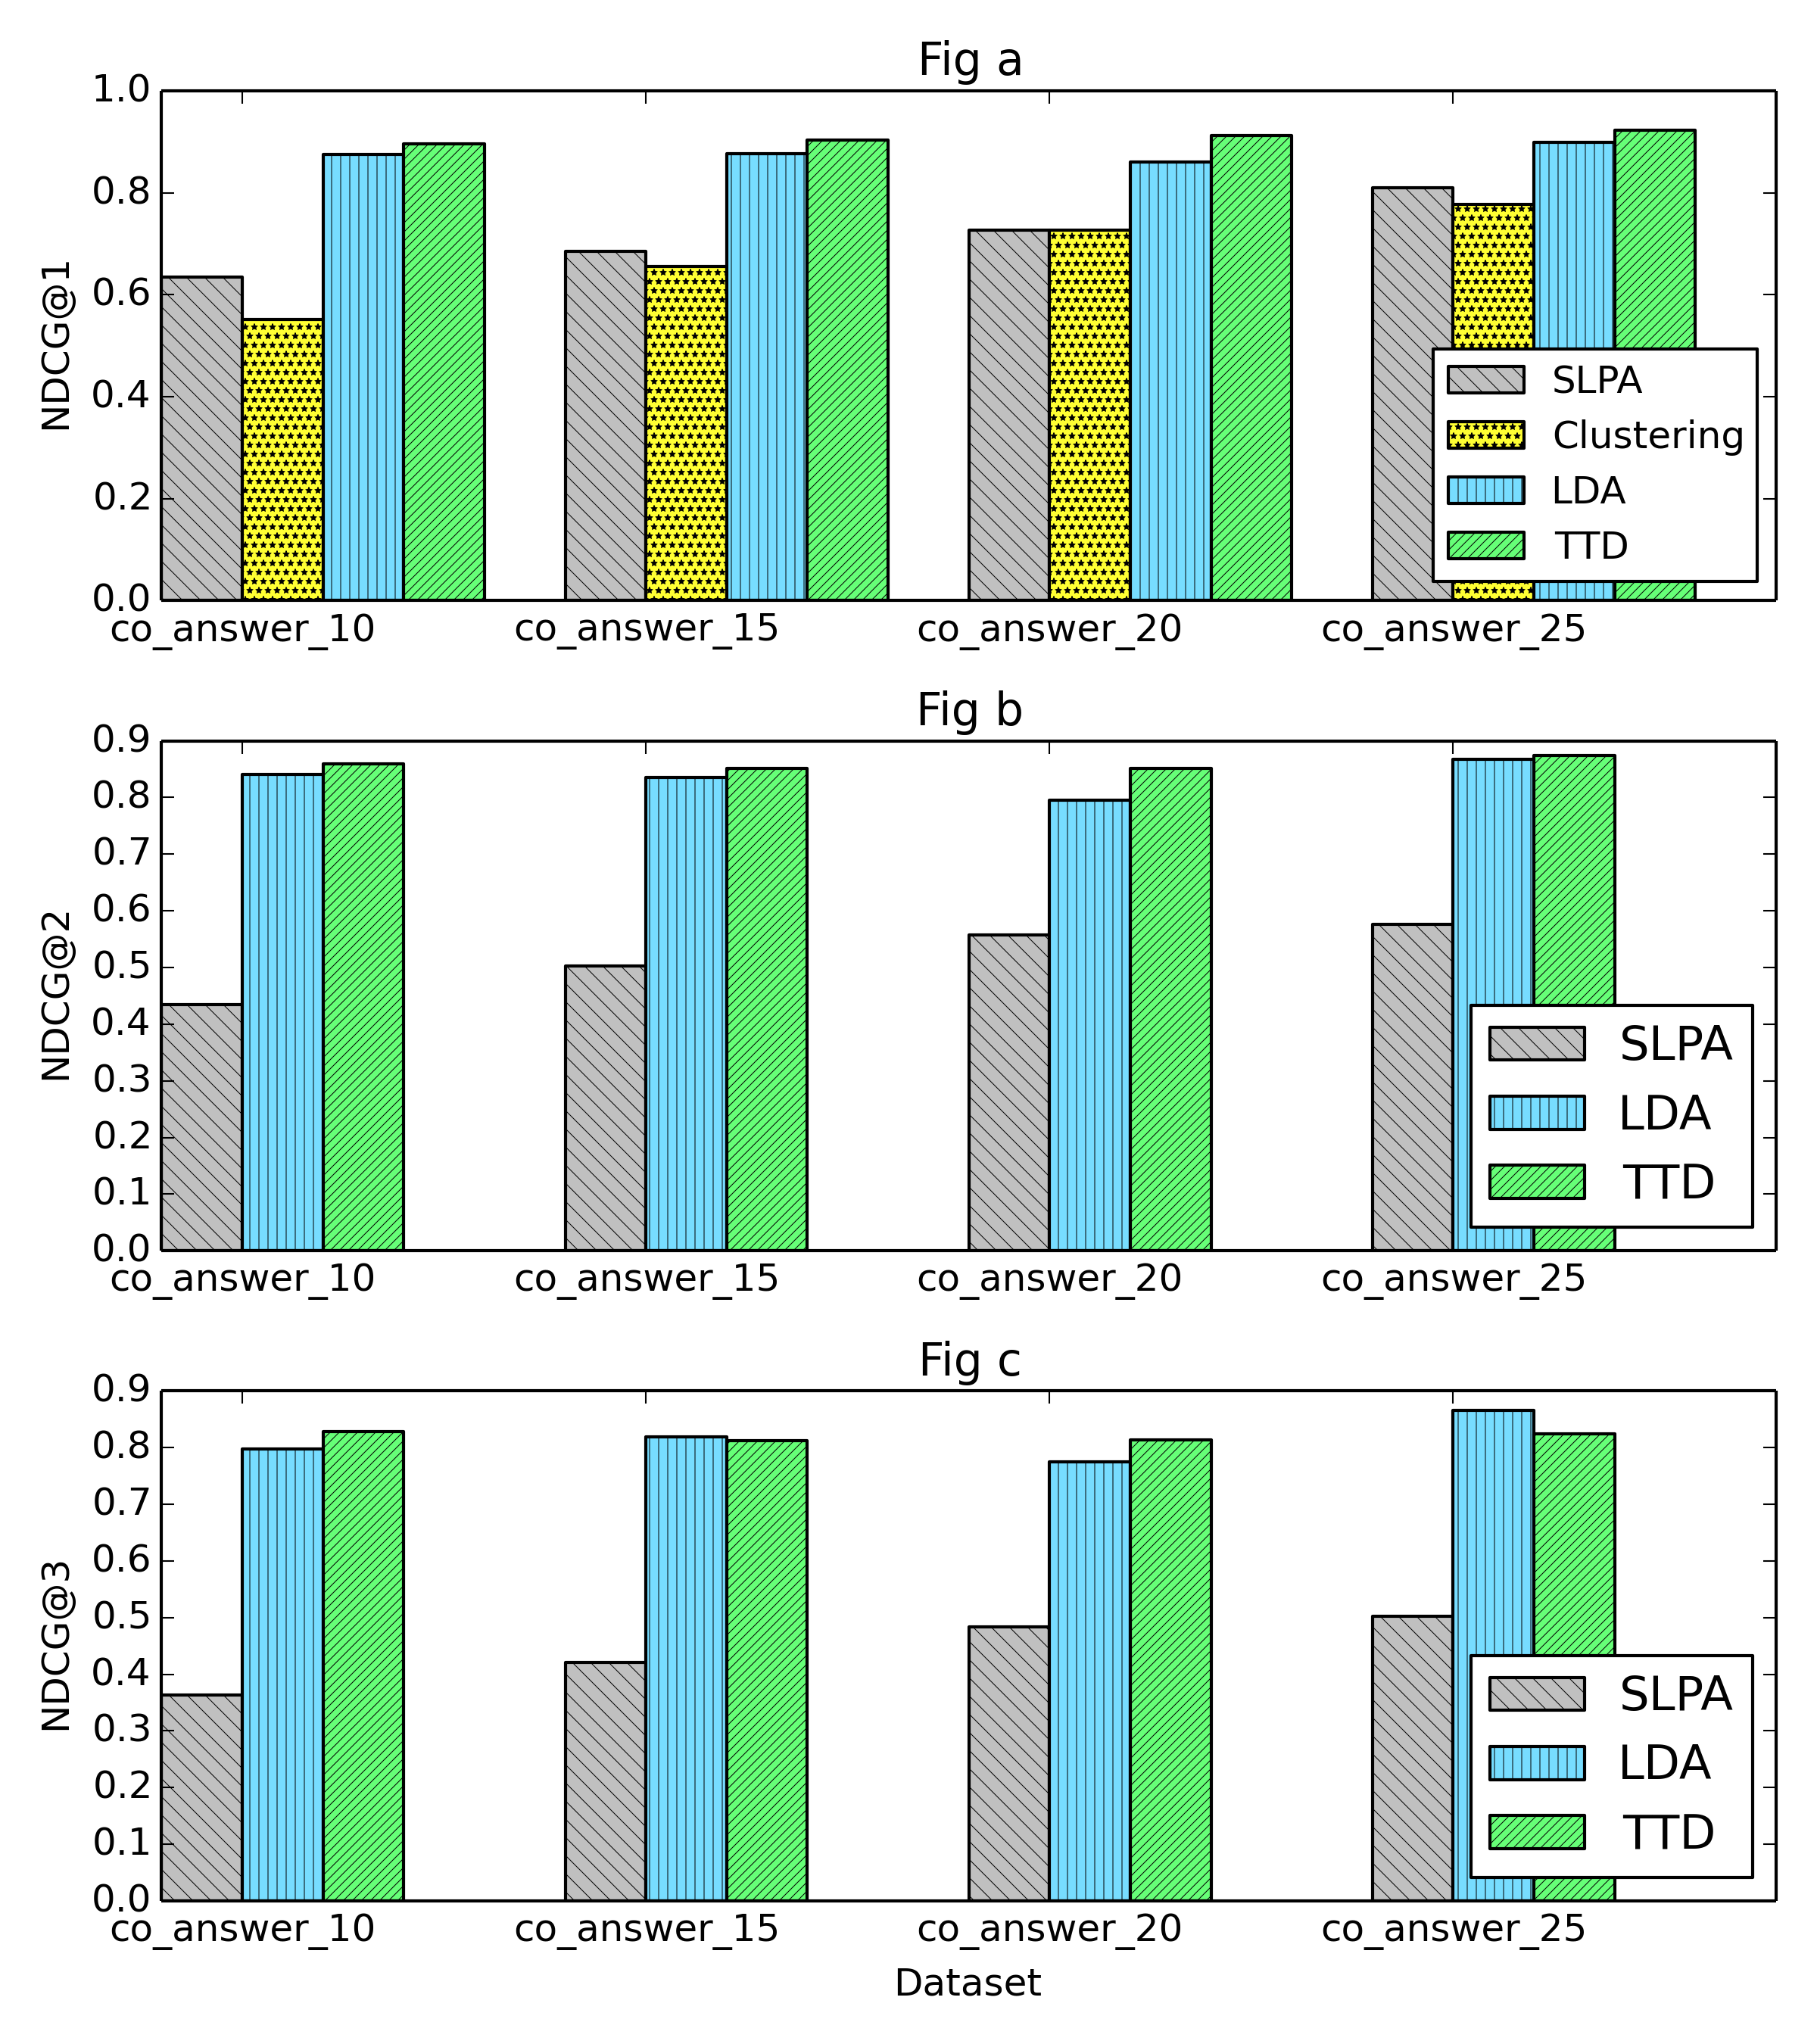
\includegraphics[width=5in]{all_in_one.png} 
\caption{NDCG results comparaison}
\label{fig:allinone} % Fig.2
\end{figure}
NDCG@1 reflects the prominent interest detected by each algorithm compared with the ground-truth of user's prominent interest. We noticed that our Empirical method is partially better than LDA, and outperforms SLPA and hierarchical clustering. We also mention that with the dataset becoming less noisy (people have prominent and clear-intention interests), all methods' performance increase. The same phenomenon is also observed in NDCG@2,3. As hierarchical clustering algorithms give a hard partition there are no performance comparison for hierarchical clustering algorithm in NDCG@2,3. Although there is limitation in the user study because that the ground-truth is the human judgement label, which may have some bias. It still worth to do this experiment because that the similarity experiment focus more on the community, but this user study experiment focus more on each user.


\subsection{Scalability: topic based user assignment is scalable}
We also evaluated the scalability of each method. However, as these methods are written in different programming languages, it is not fair to consider this as a precise evaluation; it is just an indication. To increase the stability of the comparison, we run experiments 10 times, and listed the average values. We used a Java implementation of LDA algorithm. All the other methods were implemented in Python. For our method, the time of topic detection was also counted in. For LDA and SLPA, we set the iteration number at 100. We run the experiments on a computer with 3GHz Intel i7 CPU and 8GB RAM. From the experiment, we could find that LDA, SLPA and our method are linear in terms of the number of users. Although LDA algorithm is theoretically $O(nm)$ in each iteration, with $n$ representing the number of users, and $m$ representing the number of tags for each user, when we test it on large datasets, it clearly appears that only $n$ actually has an impact; $m$ has a very low impact. So LDA could be regarded as linear. Besides, \cite{griffiths2004finding} proved that LDA model requires a few hundreds of iterations to obtain stable topic distribution. Our model does not have this limitation.
\begin{figure}[htp]\centering
%\epsfig{file=fly.eps, height=1in, width=1in}
%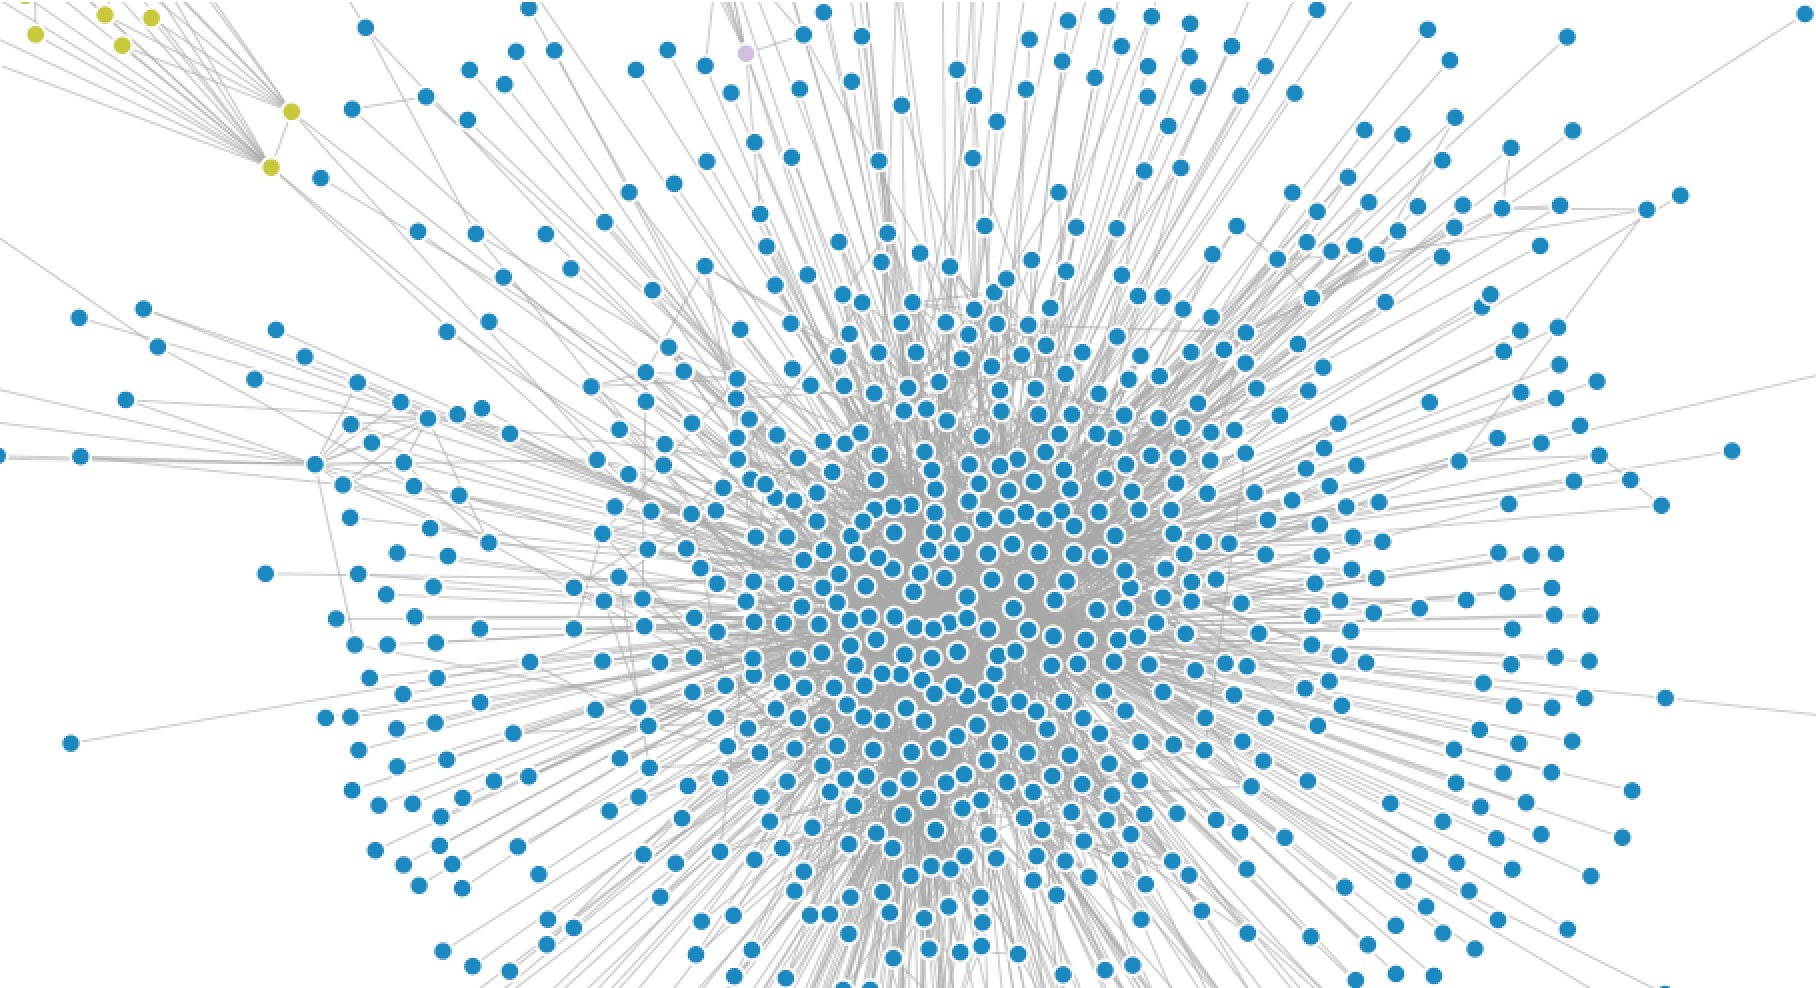
\includegraphics[height=2in, width=3.2in]{lpa_co_answer_10.png}  % use this if you use "pdflatex"
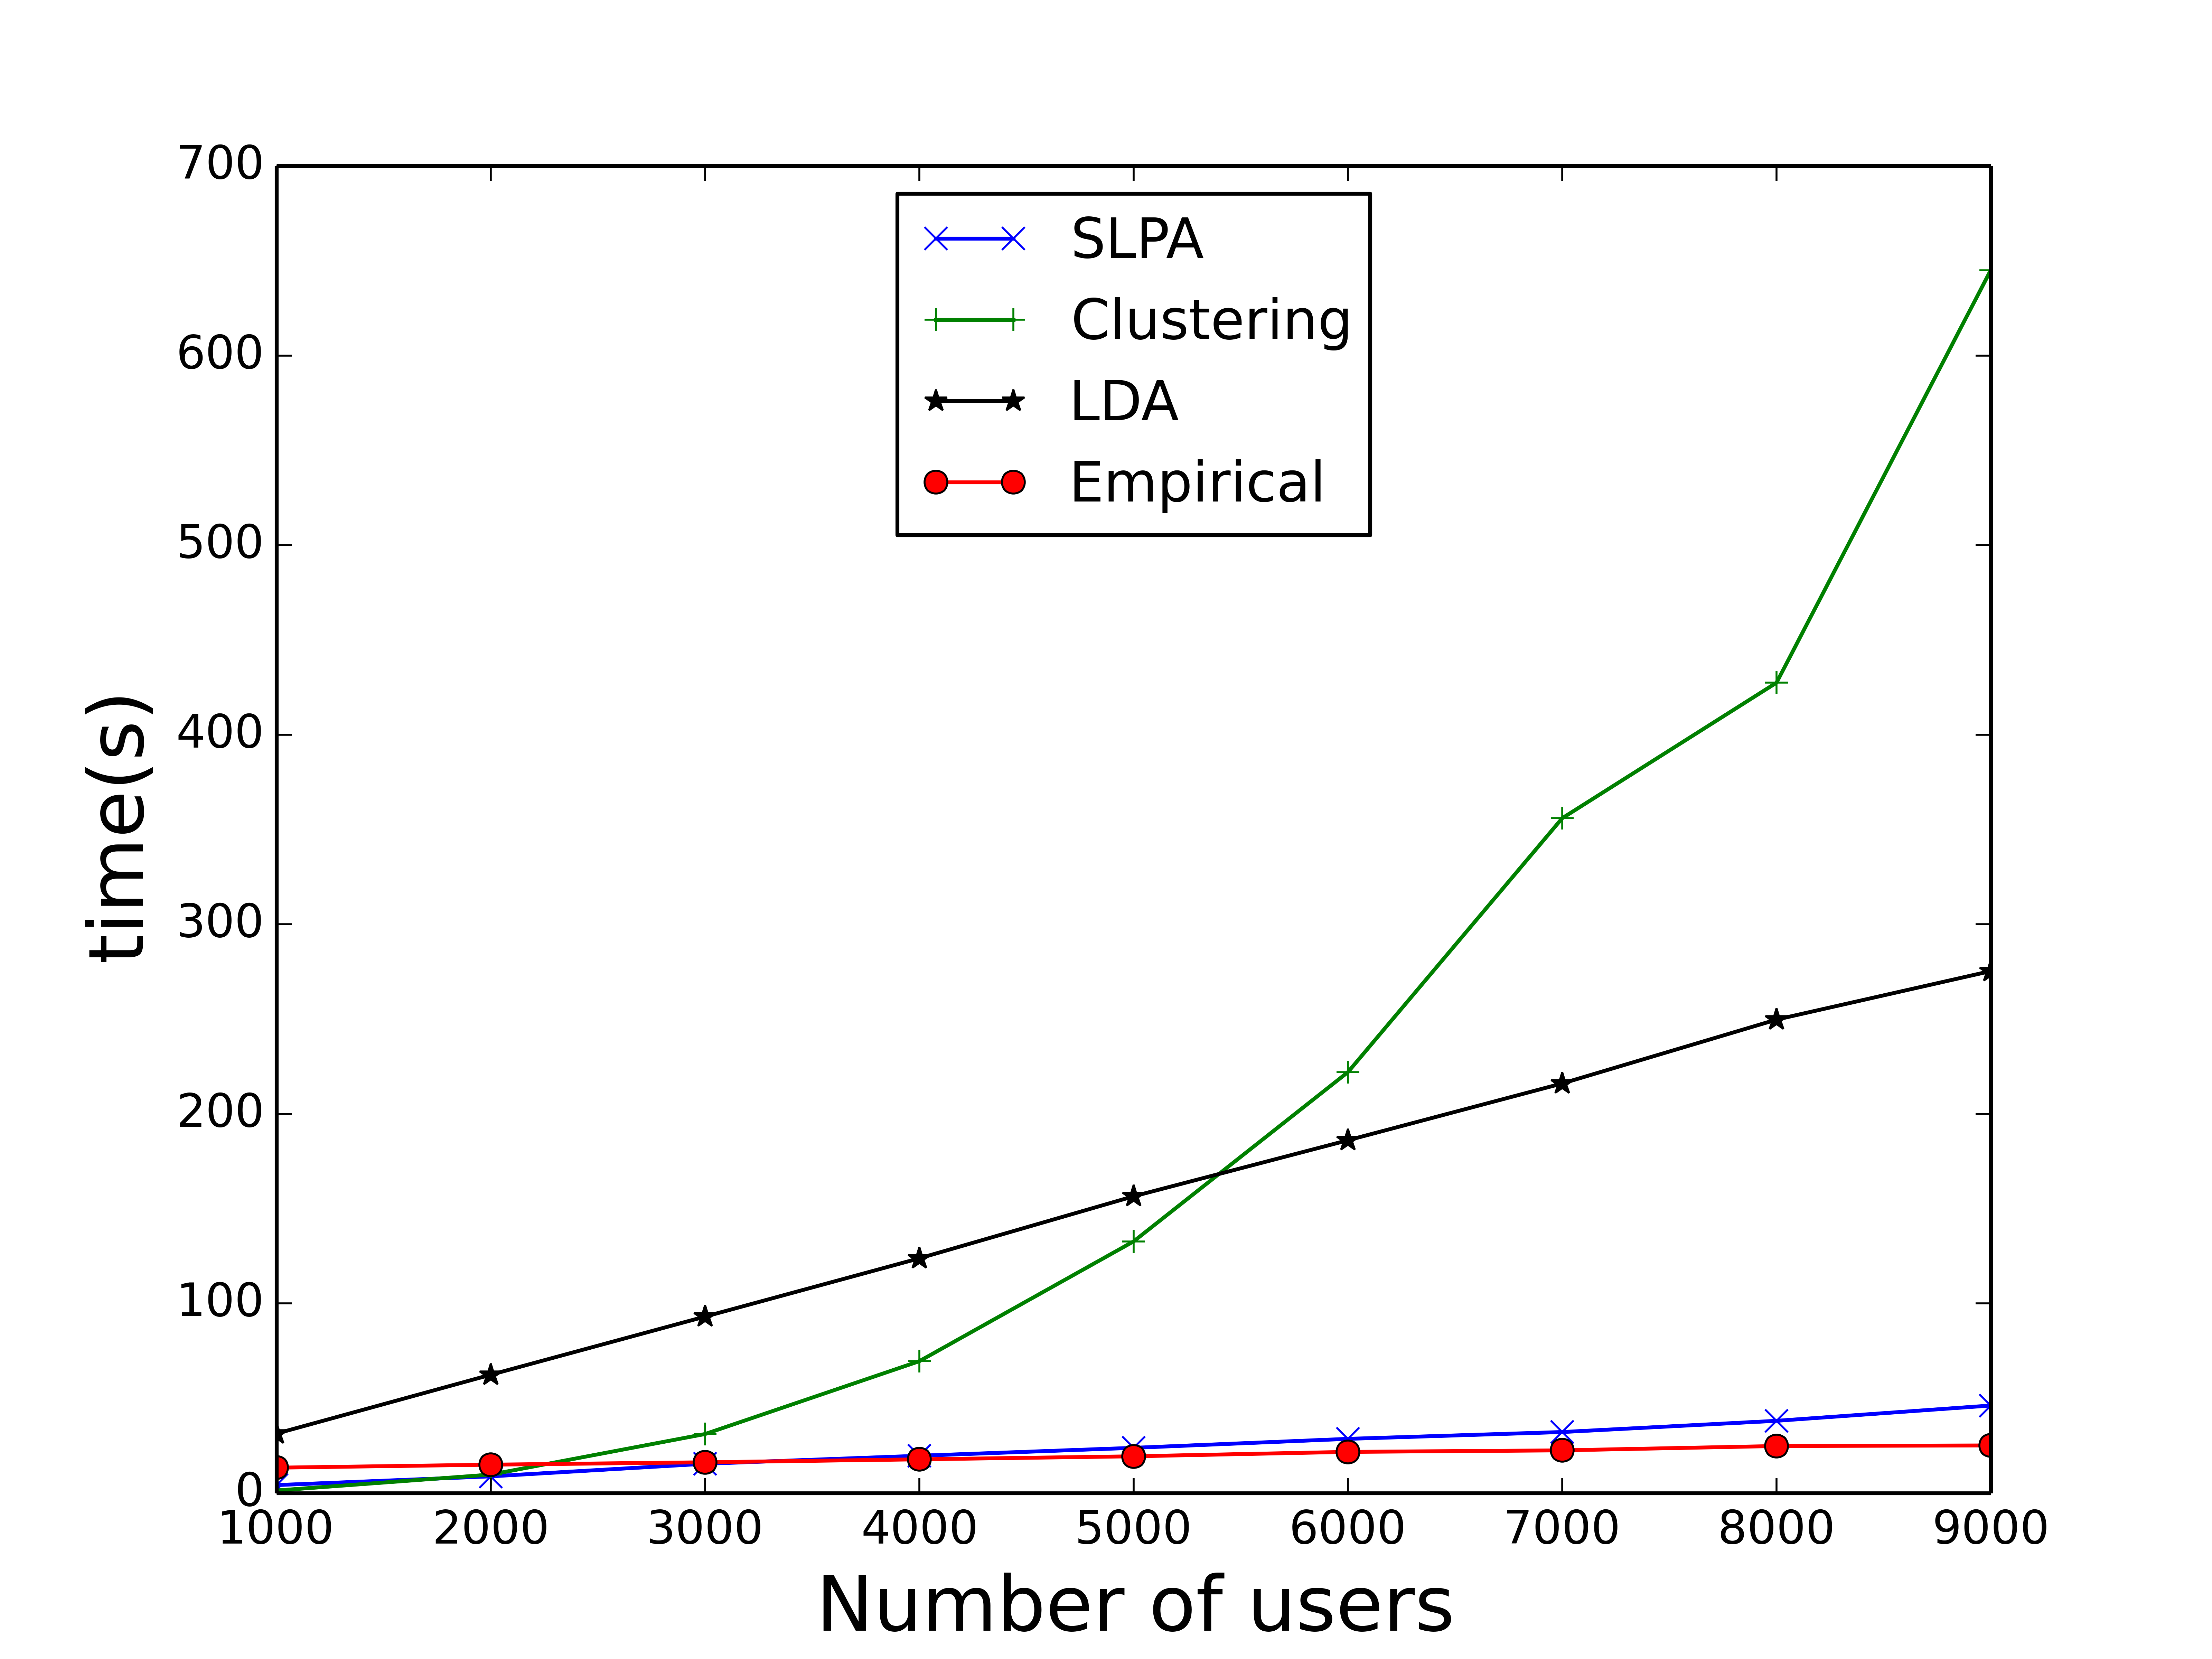
\includegraphics[width=5in]{time_perfor.jpg} 
\caption{Scalability of the compared user interest detection methods}
\label{fig:scalability} % Fig.2
\end{figure}

% TODO: you need to report your evaluation on Flickr to validate on other datasets. 
%DONE

\subsection{Genericity of the proposed Topic Extraction Method}
In order to test that whether our proposed topic extraction methods is generic, we collected a dataset from flickr\footnote{flickr website: \url{https://www.flickr.com/} } which contains 1211499 photos attached with tags. For instance, a photo tagged with \{\emph{china} \emph{pinyao}\} indicates the location information. A photo tagged with \{\emph{night} \emph{people} \emph{bar}\} describes the time and content information. We run our topic extraction method on this dataset, and we list some results in Table \ref{tab:flickrdataset}. We can find that the detected topics are interesting. For example, topic 3 includes photos which contains airplanes, topic 24 includes photos which contains bicycles, and topic 23 includes photos taken in cities of Italy.
\begin{table}[htp]
%\begin{table}[!t]
\caption{Top tags and their probabilities on flickr dataset}
\label{tab:flickrdataset}
\centering
\scriptsize
%\begin{tabular}{|p{43pt}|p{10pt}|p{37pt}|p{10pt}|p{50pt}|p{10pt}|}
\begin{tabular}{|c|c|c|c|c|c|}
\hline
\multicolumn{2}{|c|}{topic3} & \multicolumn{2}{c|}{topic4} & \multicolumn{2}{c|}{topic5}  \\
\hline
airplane&0.074&tshirt&0.216&music&0.077\\ \hline
airport&0.053&shirt&0.154&rock&0.040\\ \hline
aircraft&0.029&shirts&0.112&concert&0.036\\ \hline
flying&0.028&threadless&0.109&live&0.025\\ \hline
plane&0.027&tshirts&0.009&band&0.022\\ \hline
aviation&0.022&tee&0.008&singing&0.019\\ \hline
flight&0.014&clothing&0.007&guitar&0.018\\ \hline
aeroplane&0.012&media&0.006&festival&0.017\\ \hline
jet&0.010&models&0.006&show&0.014\\ \hline
boeing&0.009&camiseta&0.004&livemusic&0.010\\ \hline
\hline
\multicolumn{2}{|c|}{topic23} & \multicolumn{2}{c|}{topic24} & \multicolumn{2}{c|}{topic25}  \\
\hline
italy&0.179&bike&0.114&portrait&0.049\\ \hline
italia&0.053&motorcycle&0.052&girl&0.029\\ \hline
rome&0.028&racing&0.033&woman&0.014\\ \hline
florence&0.021&bicycle&0.028&smile&0.014\\ \hline
venice&0.014&race&0.027&model&0.010\\ \hline
tuscany&0.014&motorbike&0.024&sexy&0.009\\ \hline
roma&0.011&sport&0.019&face&0.008\\ \hline
europe&0.011&speedway&0.011&fun&0.008\\ \hline
firenze&0.010&500cc&0.010&man&0.008\\ \hline
milan&0.007&methanol&0.010&love&0.008\\ \hline
\end{tabular}
\end{table}




\subsection{Discussion: q\&a social network is different}
%This paragraph is used for analysis parameters. TBD
To sum up, most community detection algorithms work well on real-life social networks which contain many \textit{triangle-shape} structures. The interactions between the users in these networks are mainly based on their relationships. It is also noticeable that the relationships which a user in such network can maintain are limited and most likely restricted by the location (co-author networks in academia is also in this situation), so the overall structure of the network is \textit{flatter}, \textit{scattered} and with many \textit{triangle-shape} structures. Comparatively, in Q\&A sites, such as StackOverflow, there are no fixed relationships between users. Users interact with each other based on their own interests. And they are not aware of whom they are interacting with, so they will not maintain explicit relationships. Besides, a user can interact with any other user and mainly interacts with the \textit{"gurus"} (most of questions are answered by a small group of people). So the overall structure of the network is \textit{octopus-shape}~\cite{leskovec2008statistical} with less \textit{triangle-shape} structures. According to~\cite{park2013efficient}, the average number of \textit{triangle-shape} structures per user in Twitter dataset is around $35714$, while in our co-answer-10 dataset, the number of \textit{triangle-shape} structure per user is around $30$ which is far less. So, graph-based community detection methods fail in such situation. The result of SLPA algorithm shows that it outputs one or two giant groups, together with many tiny groups that only contain a small number of users as depicted in Figure \ref{fig:co-answer-network-10}, where each color represents a detected community. We can also see that the network contains less \textit{triangle-shape} structures and a high-density \textit{core}. It also indicates that the network has huge overlaps. However, in co-answer-25 dataset, the graph structure is more \textit{flatter} and contains many \textit{triangle-shape}. Therefore, as shown in figure \ref{fig:co-answer-network-25}, the result of SLPA algorithm outputs several medium sized groups.

% TODO: you need a longer label and a legend for this figure.
%DONE
\begin{figure}[htp]
\centering
%\epsfig{file=fly.eps, height=1in, width=1in}
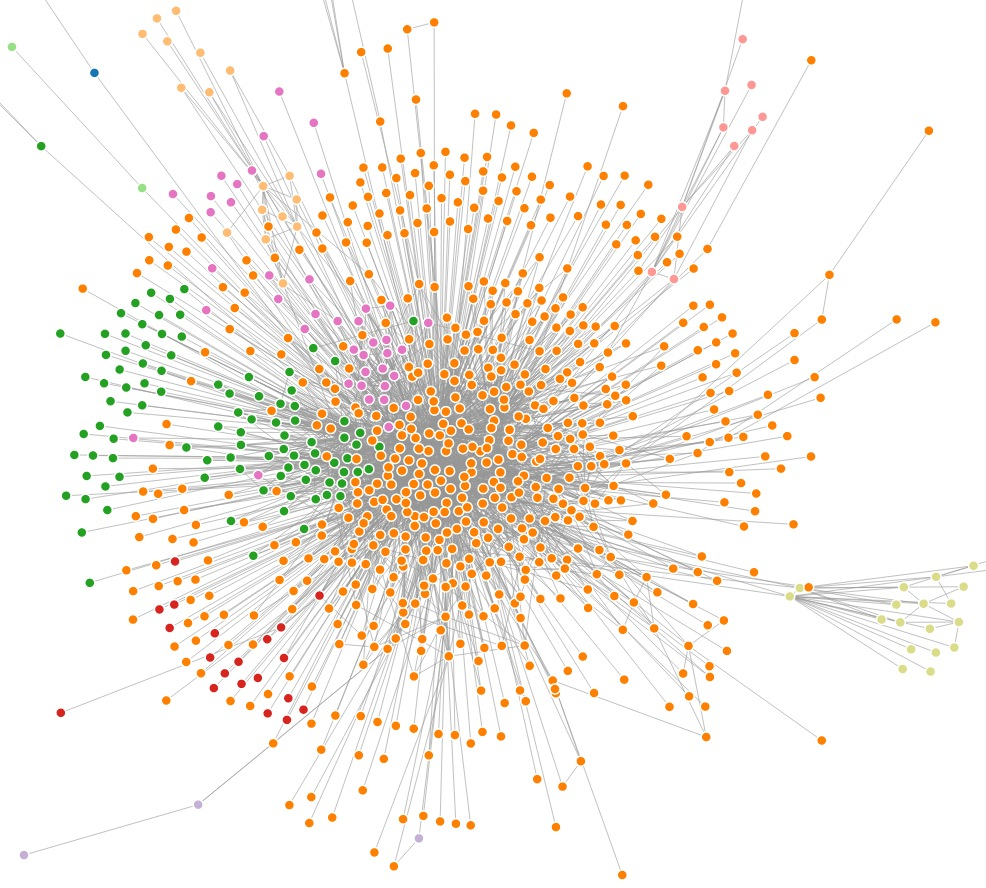
\includegraphics[width=5in]{lpa_10_V2.png}  % use this if you use "pdflatex"
\caption{Illustration of co-answer-network-10, different color indicate detected communities}
\label{fig:co-answer-network-10} % Fig.2
\end{figure}

\begin{figure}[htp]
\centering
%\epsfig{file=fly.eps, height=1in, width=1in}
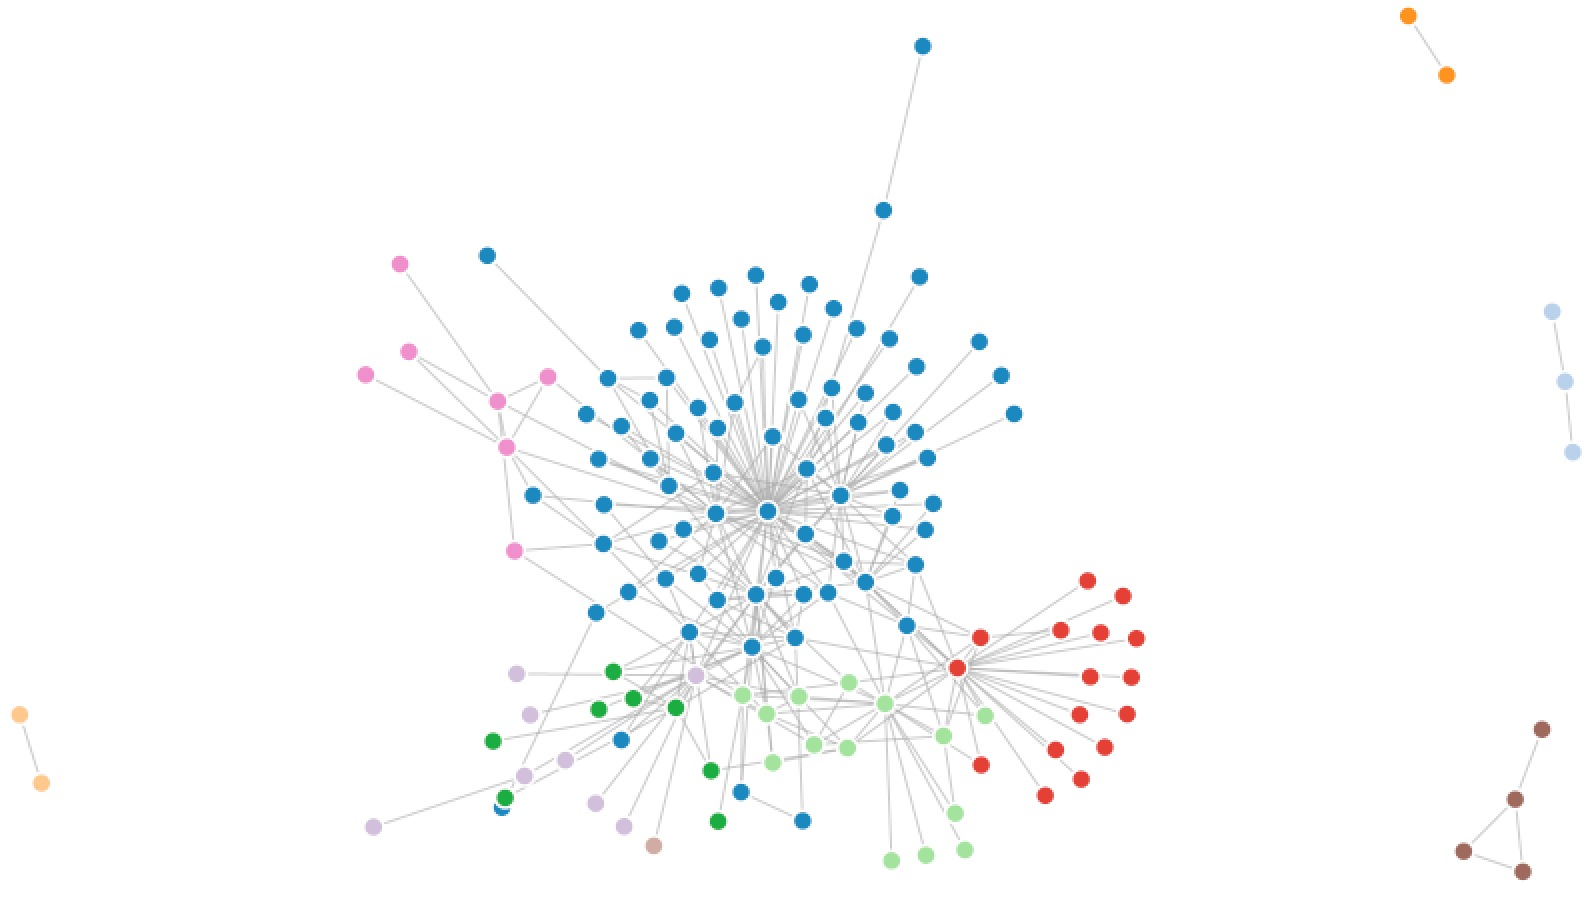
\includegraphics[width=5in]{lpa_co_answer_25.png}  % use this if you use "pdflatex"
\caption{Illustration of co-answer-network-25, different color indicate detected communities}
\label{fig:co-answer-network-25} % Fig.2
\end{figure}
Since clustering methods normally generate hard-partition communities, they cannot detect the overlapping communities which are typical in our case. Concerning the LDA-based methods, on one hand, in our dataset, question tag lists are quite short, and the experiment shows that our topic extraction method gives better results in this situation. On the other hand, the probabilistic graphical model requires hundreds of iterations to get stable results~\cite{griffiths2004finding} which is more complicated and slower than our method. 
\section{Summary: a efficient user topic extraction method}
Recalling our research questions (How can we detect communities of interests in Q\&A sites? How can we also identify the topics that attract them?) we believe that we propose a topic detection method which is very suitable for Q\&A datasets and an efficient user interest detection method to discover topic based overlapping communities of interests. As we found in the topic extraction result, the output are just bag of words with labels such as "topic 15", "topic 30", it is not easy to understand the meaning of the topic by these labels, so we try to tackle this problem in next chapter. The goal will be automatic generate a label for a bag of words.

